\section{Configuring ROMS for a Specific Application}
\label{Wave}
This chapter describes the parts of ROMS for which the user is
responsible when configuring it for a given application.  Section
\ref{User} describes the process in a generic fashion while
\S\ref{UpDown} and \S\ref{ARCTIC} step through the application of ROMS
to upwelling/downwelling and wind-driven Arctic problems,
respectively.  As distributed, ROMS is ready to run quite a few
examples, where the C preprocessor flags determine which is to be
executed.  Some of these examples are described in
\citet{Haidvogel99}, some are listed here:
\begin{klist}
   \kitem{BASIN} This is a rectangular, flat-bottomed basin with
 double-gyre wind forcing. When run, it produces a western boundary
 current flowing into a central ``Gulf Stream''
 which goes unstable and generates eddies. The goal is to run
 adiabatically to study the homogenization of potential vorticity.
 It earned its nickname of Big Bad Basin by taking a long time to
 run and causing difficulties for the spectral versions of SPEM.
%   \kitem{CANYON\_A} The canyon is a periodic channel with a steep shelf
% along one wall, where the shelf contains a steep canyon.  There is a
% periodic forcing which causes the water to oscillate along the
% channel.  The rotation and the shelf lead to non-zero mean flows,
% especially near the canyon.  Version A is homogeneous and can be
% executed with a 2-D model.  See \citet{HB97} for
% a description of the canyon problems and the gravitational adjustment
% problem.
%   \kitem{CANYON\_B} This is like Canyon A, except that it is
% stratified.
%   \kitem{DAMEE\_4}  DAMEE stands for Data Assimilation and Model
% Evaluation Experiment and is a comparison of different models of
% the North Atlantic.  Version 4 is a big domain
% extending from 30$^\circ$ S to 65$^\circ$ N.  Additional input files
% are required to run the DAMEE configurations.
   \kitem{GRAV\_ADJ} The gravitational adjustment problem takes place
 in a long narrow domain which is initialized with dense water at one
 end and light water at the other. At time zero, the water is released
 and it generates two propagating fronts as the light water rushes to
 fill the top and the dense water rushes to fill the bottom. This
 configuration can be used to test various advection schemes.
   \kitem{OVERFLOW}   This configuration is similar to the
 GRAV\_ADJ problem, but is initialized with dense water in the shallow
part of a domain with a sloping bottom.
   \kitem{SEAMOUNT}   The seamount test has been used to test the pressure
 gradient errors.  It has an idealized seamount in a periodic channel.
 See \citet{BH93} and \citet{McCalpin94} for more information.
   \kitem{UPWELLING}  The upwelling/downwelling example was
 contributed by \citet{Macks93}
 and consists of a periodic channel with shelves on each side.
 There is along-channel wind forcing and the Coriolis term leads
 to upwelling on one side and downwelling on the other side. If
 you run it for several days without vertical mixing, you end up with
 dense water over light water.
\end{klist}
Some NetCDF input files for the ROMS examples can be found under
\code{Data/ROMS} in the ROMS distribution while many others can be
downloaded as part of the \href{http://www.myroms.org/svn/src/test}{ROMS
test package}. The ASCII input files are under \code{ROMS/External}.

\subsection{Configuring ROMS}
\label{User}

The four main sections you need to change in ROMS are the \code{makefile}
or \code{build.bash}, an include file with \code{cpp} options, any
analytic functions, and the ASCII input file. If more realistic fields
are desired, you will have to provide other input files as well, for
instance for the grid and the wind forcing.

\subsubsection{Case Name}

First, you need to decide on a name for your particular application or
configuration. This name is provided via the \code{ROMS\_APPLICATION} in
either the makefile or the build script. This name should be reasonably
short, all uppercase, with spaces converted to underscores. For example,
let's say we pick the name \code{WIKI\_TEST}. This name gets defined
during the build, so you can add code protected by \code{\#ifdef
WIKI\_TEST} as needed. This would be a good time to either copy the
makefile or the build Script to create one specific to this case prior
to editing it.

\subsubsection{ Case-specific Include File}

Each application has its own include file, included by
\code{cppdefs.h}. The name of this file is the name of your
application (\code{WIKI\_TEST} here) turned into lower case, with '.h'
appended (\code{wiki\_test.h}). The location of this file is set by
\code{MY\_HEADER\_DIR}, pointing to \code{User/Include} or some other
location of your choosing.

The complete list of options to be set prior to compilation are listed in
\S\ref{Cpp1}. Place those you need in the \code{wiki\_test.h} file. These
include algorithm choices (e.g. advection and turbulence closure schemes),
output options (averages, diagnostics, stations, floats), and
application modules (biology, sediments). Each line should be of the
form:
\begin{verbatim}
        #define SOME_VAR
\end{verbatim}
Note that any undefined variable need not be mentioned.

Also note that if you copy a predefined application from
\code{ROMS/Include} as a template for your application, you must
rename it. If you don't change the name, ROMS will use the one in
\code{ROMS/Include} and your file will be ignored during the build
procedure.

\subsubsection{Functionals}

Some of the cpp options have names beginning with \code{ANA\_}. For each one of
these, you will be expected to provide an analytic expression for the field
in question in the corresponding include file. These files
are listed in \S\ref{Functionals} and their location is determined
by \code{MY\_ANALYTICAL\_DIR}. You may chose to copy those from
\code{User/Functionals} to some new directory and place your version of
the assignments within
\begin{verbatim}
        #ifdef WIKI_TEST
        ! Set weird and wonderful winds
           :
        #endif
\end{verbatim}
This makes
it easy to search for later, if nothing else.

\subsubsection{\code{checkdefs.F}}

If you add new \code{cpp} variables to the code (other than your
application name), it is recommended that you also add the appropriate
code to \code{checkdefs.F}, such as:
\begin{verbatim}
       #ifdef SLEET
             IF (Master) WRITE(stdout,20) 'SLEET',                      &
            &   'Sleet falling on the ice option.'
             is=lenstr(Coptions)+1
             Coptions(is:is+7)=' SLEET,'
       #endif /* SLEET */
\end{verbatim}
Note that the number ``7'' on the \code{Coptions} line must be set
according to the length of the string you are adding.  In this case 7
is for `` SLEET,'', including the comma and the space. You do not
need to do this for your application name (\code{WIKI\_TEST} here),
since \code{checkdefs} will print whatever is in \code{MyAppCPP}.

\subsubsection{Model domain}
\label{Muddy}
It is assumed in this manual that \code{Ngrids} will be set to 1.
Having multiple grids talk to each other is brand new in ROMS 3.7,
with documentation appearing on the ROMS wiki.

One of the first things the user must decide is how many grid points
to use, and can be afforded.  There are three parameters in
\code{ocean.in} which specify the grid size and one parameter for the
number of active tracers:
\begin{tabbing}
  Gnu \= Allolo \= \kill
  \> \code{Lm} \> Number of finite-difference points in $\xi$. \\
  \> \code{Mm} \> Number of finite-difference points in $\eta$. \\
  \> \code{N} \> Number of finite-difference points in the vertical. \\
  \> \code{NAT} \> Number of active tracers. \\
\end{tabbing}
The number of biological tracers is set in the \code{biology.in} file.
There are no constraints on these except $\code{Lm} \geq 2$, $\code{Mm}
\geq 2$, $\code{N} \geq 2$ and $\code{NAT} \geq 1$.  \code{Lm} and
\code{Mm} should be at least 3 if the domain is periodic in that
direction.

\subsubsection{$x,y$ grid}
The subroutine \code{get\_grid} or \code{ana\_grid} is called by
\code{initial} to set the grid arrays, the bathymetry, and the
Coriolis parameter.  Most of the simple test problems have their grid
information specified in \code{ana\_grid.h} in the directory
\code{ROMS/Functionals}.  More realistic problems require a NetCDF grid
file, produced by the grid generation programs described in
\citet{GRIDS}, by the Matlab \code{SeaGrid}, or by some
other method.  The variables which are read by \code{get\_grid} are:
\begin{tabbing}
  Gnu \= \kill
  \> \code{xl, el, spherical, f, h, pm, pn, x\_rho, y\_rho,
  lon\_rho, lat\_rho, angle}.
\end{tabbing}
If the grid is curved, \code{get\_grid} will also read:
\begin{tabbing}
  Gnu \= \kill
  \> \code{dndx, dmde}.
\end{tabbing}
Likewise, if \code{MASKING} is defined, it will read:
\begin{tabbing}
  Gnu \= \kill
  \> \code{mask\_rho, mask\_u, mask\_v, mask\_psi}.
\end{tabbing}

\subsubsection {$\xi,\eta$ grid}
Before providing initial conditions and boundary conditions, the
user must understand the model grid. The fields are laid out on an
Arakawa C grid as in Fig.\ \ref{fcgr}. The overall grid is shown in
Fig.\ \ref{fwgr}.  The thick outer line shows the position of the
model boundary. The points inside this boundary are those which are
advanced in time using the model physics. The points on the boundary
and those on the outside must be supplied by the boundary
conditions.

The three-dimensional model fields are carried in four-dimensional
arrays, where the fourth array index refers to one of two or three
time levels. The tracers have a fifth array index telling which
tracer is being referred to.
For instance, $\code{itemp}=1$ refers to
potential temperature while $\code{isalt}=2$ refers to salinity.  The
integers $i$, $j$, and $k$ are used throughout the model to index
the three spatial dimensions:
\begin{tabbing}
Gnus \= Gnus \= \kill
   \>$i$ \>Index variable for the $\xi$-direction. \\
   \>$j$ \>Index variable for the $\eta$-direction. \\
   \>$k$ \>Index variable for the $\sigma$-direction.  $k = 1$
   refers to the bottom \\
biggnu \= \kill
   \>while $k = \code{N}$ refers to the surface.
\end{tabbing}

%The range of $\xi$ is 1 to \code{L} and the range of $\eta$ is 1 to
%\code{M}.  Therefore $i$ and $\xi$ are the same at $\psi$
%points, as are $j$ and $\eta$.  (This matters in the floats---Dale and
%I disagreed on how this should be and then Dale later changed to my
%point of view after I had recoded things to match his).

\subsubsection{Initial conditions}
The initial values for the model fields are provided by either
\code{ana\_initial} or \code{get\_state}.  \code{get\_state} is
also used to read a restart file if the model is being restarted from a
previous run.

Also in \code{initial}, \code{rho\_eos} is called to initialize
the density field. \code{rho\_eos} also computes \code{rhoA},
the vertically averaged density, and \code{rhoS}, the density
perturbation. Both \code{rhoA} and \code{rhoS} are used in the barotropic
pressure gradient.

%The tracer climatology fields also require appropriate values if they
%are to be used, and are provided by \code{ana\_tclima} or
%\code{get\_tclima}. Likewise, the surface height climatology is read by
%\code{get\_ssh} or provided by \code{ana\_ssh}.

\subsubsection{Equation of state}
The equation of state is defined in the subroutine \code{rho\_eos}.  Two
versions are provided in ROMS: a nonlinear $\rho =
\rho(T,S,z)$ from \citet{Jackett} and a linear
$\rho(T,S)$.  The linear form is
$$
      \rho = \code{R0} - \code{Tcoef} \cdot (T-T0) +
      \code{Scoef} \cdot (S-S0)
$$
or
$$
     \rho = \code{R0} + \code{Tcoef} \cdot (T-T0),
$$
depending on whether or not
\code{SALINITY} is defined.  Specify which equation of state you
would like to use with the \code{NONLIN\_EOS} C preprocessor flag in your
application include file. The linear coefficients \code{R0}, \code{T0},
\code{Tcoef}, \code{S0}, and \code{Scoef} are set in \code{ocean.in}. Note
that we are computing {\em in situ} density from potential temperature and
salinity. Some of the vertical mixing schemes require potential density
and some other fields, which are computed by \code{rho\_eos} as well.

\subsubsection{Boundary conditions}
\label{Bcs}
The horizontal boundary conditions are provided by the subroutines
in \code{u3dbc\_im}, \code{v3dbc\_im}, \code{u2dbc\_im}, \code{v2dbc\_im},
\code{t3dbc\_im}, and \code{zetabc}.  They are called every time-step
and provide the boundary values for the fields $u, v, \overline{u},
\overline{v}$, all tracers, and $\zeta$, respectively. They are currently
configured for a closed basin, a periodic channel, a doubly periodic
domain or a domain with various open boundary conditions. Each side is
controlled independently with ``West'' being the \code{i=1} boundary,
``East'' being the \code{i=L} boundary, ``South'' being the \code{j=1}
boundary, and ``North'' being the \code{j=M} boundary. These choices are
set in \code{ocean.in} via the \code{LBC} array.

Many of the choices for open boundaries require that the model have
some boundary values for the field in question. These can be specified in
the appropriate \code{ana\_xxx.h} file for say \code{ANA\_TOBC} or
they can be read from a boundary NetCDF file. There is logic in
\code{globaldefs.h} by which ROMS decides whether or not it needs to
read a boundary file.

\subsubsection{Model forcing}
\label{Mforce}
\noindent {\bf(a) Winds and thermal fluxes}

There are two different ways to apply a wind forcing: as a surface
momentum flux in the vertical viscosity term, or as a body force over
the upper water column.
Usually, we set the vertical $\sigma$-coordinate
parameters to retain some resolution near the surface and apply the
fluxes as boundary conditions to the vertical viscosity/diffusivity.
In either case, the surface and bottom fluxes are either defined
analytically, read from a forcing file, or computed inside ROMS
using a bulk flux formula from the appropriate atmospheric fields
(air temperature and winds, for instance).  You must either edit the
appropriate \code{ana\_xxx.h} or create a NetCDF forcing
file in the format expected by ROMS. Note that it is quite common
to put the surface variables in the forcing file while having an analytic
bottom heat flux. ROMS now has the capability of reading in a list
of forcing fields---it can be convenient to have one file per field
rather than stuffing tides, winds, river inputs all into one file.

In the past, our vertical resolution was relatively coarse and the
vertical viscosity would have to have been unreasonably large for
us to resolve the surface Ekman layer.  If that is your situation,
define \code{BODYFORCE} in \code{cppdefs.h} and provide a value for
\code{levsfrc} in \code{ocean.in}.  The forcing is applied over the
levels from \code{levsfrc} to \code{N}.  The above caution about
vertical resolution also applies to the surface fluxes of $T$ and
$S$, although \code{BODYFORCE} only refers to wind stress, not the
surface tracer fluxes.

\smallskip
\noindent {\bf(b) Climatology}

One way to force the model is via a nudging to the tracer and/or
momentum climatologies. Nudging to tracers was used in the North
Atlantic simulations in sponge layers along the northern and southern
boundaries. Set the climatologies in \code{ana\_tclima.h} or in a
file read by \code{get\_data}, set \code{LtracerCLM} in
\code{ocean\_wiki\_test.in} and also set the array \code{Tnudgcof} in
either \code{ana\_nudgcoef.h} or in a file (with name in \code{NUDNAME}
variable in the ocean.in).

\smallskip
\noindent {\bf(c) Tides}

There is also more than one way to force with tides. One way is to
provide boundary conditions with enough temporal resolution to
resolve the tides. Another is to provide ROMS with the tidal
constituents at all grid points and to have ROMS reconstruct the
tidal currents (\code{UV\_TIDES})  and/or elevations (\code{SSH\_TIDES})
for any given time. An example of such a tidal forcing file is in
\code{Data/ROMS/Forcing/test\_head\_frc.nc}.

The non-trunk code with ice, etc. includes the \code{TIDES\_ASTRO} option to
add on the long-period tides from
\citet{Foreman_96a} and \citet{Foreman_96b}.
There is also an option to include the tidal potential
forcing term (\code{POT\_TIDES}), requiring the tidal potential to
be included in the tides forcing file.

\smallskip
\noindent {\bf(d) Rivers}

Point sources can be used to provide river inflow to the model.
These too can be specified in a forcing file if not provided via
\code{ana\_psource}.

\subsubsection{\code{ocean.in}}
\label{ASCII_in}
ROMS expects to read a number of variables from an ASCII file as described
in \S\ref{Running}.
Example input files are in \code{ROMS/External} with names like
\code{ocean\_grav\_adj.in}, where ``grav\_adj'' refers to the name of
the application. Lines beginning with ``!'' are comments and will be
ignored by ROMS on reading them.

The input is organized as key/value pairs, separated by one or two
equals signs. It is possible for ROMS to run on more than one grid
simultaneously, with the number of grids being read from the input
file. If there is one equals sign (\code{=}), ROMS will use the
corresponding value for all grids. If there are two (\code{==}), ROMS
will read a value for each grid. Thus far, our domains have used just
one grid since the inter-grid coupling has only been released very
recently.

ROMS will ignore the parameters not needed by the current simulation,
e.g., the GLS parameters will not be read if you are not using that
mixing scheme. Most of the example files contain all possible
parameters, with \code{User/External/ocean.in} being for sure updated
with each addition. The parameters are described in comments at the
bottom of the \code{ocean.in} files. Skipping those having to do
with data assimilation, the input parameters are as follows:
\begin{klist}
   \kitem{Header} \mbox{}
     \begin{klist}
   \kitem{TITLE} A text string to put in the output files.
   \kitem{MyAppCPP} The shorthand name for this application.
   \kitem{VARNAME} The location of the \code{varinfo.dat} file
     containing information about fields to read/write from/to NetCDF
     files.
   \kitem{Ngrids} The number of grids to compute on.
   \kitem{NestLayers} The number of levels of nested grids.
   \kitem{GridsInLayer} The number of grids in each nesting level.
     \end{klist}
   \kitem{Grid-dimension parameters} \mbox{}
     \begin{klist}
       \kitem{Lm} Number of $i$-direction INTERIOR RHO-points.
       \kitem{Mm} Number of $j$-direction INTERIOR RHO-points.
       \kitem{N} Number of vertical levels.
       \kitem{Nbed} Number of sediment bed layers.
       \kitem{NAT} Number of active tracers (usually 2).
       \kitem{NPT} Number of passive tracers.
       \kitem{NCS} Number of cohesive (mud) sediment tracers.
       \kitem{NNS} Number of non-cohesive (sand) sediment tracers.
     \end{klist}
   \kitem{Domain-decomposition parameters} \mbox{}
     \begin{klist}
       \kitem{NtileI} Number of $i$-direction partitions.
       \kitem{NtileJ} Number of $j$-direction partitions.
     \end{klist}
   \kitem{Boundary conditions} \mbox{}
     \begin{klist}
       \kitem{LBC} A line is given for each field, each line
       containing four values, one for each side in the order
       ``West'', ``South'', ``East'', ``North''. Each value is a
       string, with the possible values being:
         \begin{klist}
           \kitem{Cha}   Chapman implicit.
           \kitem{Che}   Chapman explicit.
           \kitem{Cla}   Clamped.
           \kitem{Clo}   Closed.
           \kitem{Fla}   Flather.
           \kitem{Gra}   Gradient.
           \kitem{Mix}   Ice only---mixed clamped and radiation.
           \kitem{Nes}   Nested.
           \kitem{Per}   Periodic---should match the opposing
boundary.
           \kitem{Rad}   Radiation.
           \kitem{RadNud}Radiation and nudging.
           \kitem{Red}   Reduced Physics---note that this also
requires the \code{FSOBC\_REDUCED} cpp flag.
           \kitem{Shc}   Schepetkin.
         \end{klist}
       \kitem{VolCons} Four values for the volume conservation, one
for each edge.
     \end{klist}
   \kitem{Time-stepping parameters} \mbox{}
     \begin{klist}
       \kitem{NTIMES}    Number of time-steps to evolve the 3-D
       equations in the current run.  This is actually the total
     number, including any previous segments of the same run.  For
     instance, if you already did a three-month run and wish to
     continue for another three months, set \code{NTIMES} to the
     number of steps needed for six months.
       \kitem{DT}        Time-step in seconds for the 3-D equations.
       \kitem{NDTFAST}   Number of time-steps for the 2-D equations
     to be executed each \code{dt}. This is the number shown as $M$
     in Figure \ref{ftspl}---the model will compute $M^\ast$ at run
     time.
     \end{klist}
%   \kitem{Model iteration loops parameters} \mbox{}
%     \begin{klist}
%       \kitem{ERstr} Starting ensemble run number.
%       \kitem{ERend} Ending ensemble run number.
%       \kitem{Nouter} Maximum number of 4DVAR outer loop iterations.
%       \kitem{Ninner} Maximum number of 4DVAR inner loop iterations.
%       \kitem{Nintervals} Number of time interval divisions for
%       stochastic optimals computations.
%     \end{klist}
%   \kitem{Generalized Stability Theory (GST) parameters} \mbox{}
%     \begin{klist}
%       \kitem{NEV} Number of eigenvalues.
%       \kitem{NCV} Number of eigenvectors.
%     \end{klist}
   \kitem{Input/Output parameters} \mbox{}

   ROMS has several possible output files. The output files can
   include a restart file, a history file, an averages file, and a
   station file, for instance.  The restart file often contains
   only two records with the older record being overwritten during
   the next write.  The history file can contain a subset of the
   restart fields, for instance just the surface elevation and the
   surface temperature.  The averages file contains time-averages
   of the model fields, for instance daily or monthly means,
   depending on \code{NAVG}.  The station file contains timeseries
   for specified points, possibly quite frequently since each record
   is small. For some, machinery is in place to write multiple
   files, numbering them \_0001, \_0002, etc.
     \begin{klist}
       \kitem{NRREC}     Record number of the restart file to read
     as the initial conditions. Set to 0 at the beginning of the
     run, -1 to read the latest record.
       \kitem{LcycleRST} Logical, true to cycle between two records
     of the restart file.
       \kitem{NRST}      Number of time-steps between writing of
     restart fields.
       \kitem{NSTA}      Number of time-steps between writing fields
     into the stations file.
       \kitem{NFLT}      Number of time-steps between writing fields
     into the floats file.
       \kitem{NINFO}     Number of time-steps between calling
       \code{diag} to write some global information and to check for
       NaN values. 
     \end{klist}
   \kitem{History, average, diagnostic output parameters} \mbox{}
     \begin{klist}
       \kitem{LDEFOUT} True for creating new output files for
     stations, history, floats, etc. If false, output is appended
     to these files.
       \kitem{NHIS}  Number of time-steps between writing history
     records.
       \kitem{NDEFHIS}  Number of time-steps between starting new history
     files.
       \kitem{NHIS2}  Number of time-steps between writing secondary
     history records.
       \kitem{NDEFHIS2}  Number of time-steps between starting new
     secondary history files.
       \kitem{NTSAVG}    Starting time-step for the accumulation of
     output time-averaged data.  For instance, you might want to average
     over the last day of a thirty-day run.
       \kitem{NAVG}      Number of time-steps between writing
     time-averaged data into the averages file.
       \kitem{NDEFAVG}      Number of time-steps between starting
     new averages files.
       \kitem{NTSAVG2}    Starting time-step for the accumulation of
     output secondary time-averaged data.  For instance, you might
     want to average over the last day of a thirty-day run.
       \kitem{NAVG2}      Number of time-steps between writing
     time-averaged data into the secondary averages file.
       \kitem{NDEFAVG2}      Number of time-steps between starting
     new secondary averages files.
       \kitem{NTSDIA}    Starting time-step for the accumulation of
     output diagnostics data.  For instance, you might want to write
     diagnostics for the last day of a thirty-day run.
       \kitem{NDIA}      Number of time-steps between writing
     diagnostics data into the diagnostics file.
       \kitem{NDEFDIA}      Number of time-steps between starting
     new diagnostics files.
     \end{klist}
%    \kitem{Tangent linear and adjoint output parameters} \mbox{}
%     \begin{klist}
%       \kitem{LcycleTLM} Logical, true to cycle between two records
%       \kitem{NTLM}      Number of time-steps between writing
%     tangent linear data.
%       \kitem{NDEFTLM}      Number of time-steps between starting
%     new tangent linear files.
%       \kitem{LcycleADJ} Logical, true to cycle between two records
%     of the restart file.
%       \kitem{NADJ}      Number of time-steps between writing
%     adjoint data.
%       \kitem{NDEFADJ}      Number of time-steps between starting
%     new adjoint files.
%       \kitem{NSFF}     Number of time-steps between 4DVAR adjustment of
%       surface forcing fluxes.
%       \kitem{NOBC}    Number of time-steps between 4DVAR adjustment of
%       open boundary fields.
%     \end{klist}
%    \kitem{Check-pointing GST restart parameters} \mbox{}
%     \begin{klist}
%       \kitem{LrstGST} GST restart switch.
%       \kitem{MaxIterGST} Maximum number of iterations.
%       \kitem{NGST} Check-pointing interval.
%     \end{klist}
%    \kitem{Ritz GST parameter} \mbox{}
%     \begin{klist}
%       \kitem{Ritz\_tol} Relative accuracy of the Ritz values
%       computed in the GST analysis.
%     \end{klist}
   \kitem{Horizontal mixing of tracers} \mbox{}
     \begin{klist}
       \kitem{TNU2}     Constant mixing
     coefficient for the horizontal Laplacian diffusion of each tracer.
     A value is expected for each of the \code{NAT+NPT} tracers.
       \kitem{TNU4}     Constant mixing
     coefficient for the horizontal biharmonic diffusion of each tracer.
     A value is expected for each of the \code{NAT+NPT} tracers.
     \end{klist}
   \kitem{Horizontal viscosity coefficients} \mbox{}
     \begin{klist}
       \kitem{VISC2}    Constant mixing coefficient for the horizontal
     Laplacian viscosity.
       \kitem{VISC4}    Constant mixing coefficient for the horizontal
     biharmonic viscosity.
     \end{klist}
   \kitem{Horizontal sponge} \mbox{}
     \begin{klist}
       \kitem{LuvSponge}   Logical for applying a sponge (increased
     horizontal viscosity) to momentum fields.
       \kitem{LtracerSponge}  Logical for applying a sponge
     (increased horizontal diffusivity) to tracer fields.
     \end{klist}
   \kitem{Vertical mixing coefficients for tracers} \mbox{}
     \begin{klist}
       \kitem{AKT\_BAK}  Background vertical mixing coefficient
     for the tracers (\code{NAT+NPT} values).
     \end{klist}
   \kitem{Vertical mixing coefficient for momentum} \mbox{}
     \begin{klist}
       \kitem{AKV\_BAK}  Background vertical mixing coefficient 
     for momentum.
     \end{klist}
   \kitem{Turbulent closure parameters} \mbox{}
     \begin{klist}
       \kitem{AKK\_BAK}  Background vertical mixing coefficient
     for turbulent kinetic energy.
       \kitem{AKP\_BAK}  Background vertical mixing coefficient
     for turbulent generic statistical field.
       \kitem{TKENU2}    Constant mixing coefficient for the horizontal
     Laplacian diffusion of turbulent kinetic energy.
       \kitem{TKENU4}    Constant mixing coefficient for the horizontal
     biharmonic diffusion of turbulent kinetic energy.
     \end{klist}
   \kitem{Generic length-scale turbulence closure parameters}
   \mbox{}
     \begin{klist}
       \kitem{GLS\_P}   Stability exponent.
       \kitem{GLS\_M}   Turbulent kinetic energy exponent.
       \kitem{GLS\_N}   Turbulent length scale exponent.
       \kitem{GLS\_Kmin}  Minimum value of specific turbulent kinetic
       energy.
       \kitem{GLS\_Pmin}  Minimum value of dissipation.
       \kitem{GLS\_CMU0}   Stability coefficient.
       \kitem{GLS\_C1}   Shear production coefficient.
       \kitem{GLS\_C2}   Dissipation coefficient.
       \kitem{GLS\_C3M}   Buoyancy production coefficient (minus).
       \kitem{GLS\_C3P}   Buoyancy production coefficient (plus).
       \kitem{GLS\_SIGK} Constant Schmidt number (non-dimensional) for
       turbulent kinetic energy diffusivity.
       \kitem{GLS\_SIGP}  Constant Schmidt number (non-dimensional) for
       turbulent generic statistical field, ``psi''.
     \end{klist}
   \kitem{Constants used in surface TKE flux computation} \mbox{}
     \begin{klist}
       \kitem{CHARNOK\_ALPHA} Charnok surface roughness.
       \kitem{ZOS\_HSIG\_ALPHA} Roughness from wave amplitude.
       \kitem{SZ\_ALPHA} Roughness from wave dissipation.
       \kitem{CRGBAN\_CW} Craig and Banner wave breaking.
     \end{klist}
   \kitem{Bottom drag coefficients} \mbox{}
     \begin{klist}
       \kitem{RDRG}     Linear bottom drag coefficient.
       \kitem{RDRG2}    Quadratic bottom drag coefficient.
       \kitem{Zob}       Bottom roughness.
       \kitem{Zos}       Surface roughness (under ice shelves).
     \end{klist}
   \kitem{Height of atmospheric measurements for bulk flux
   parameterizations} \mbox{}
     \begin{klist}
       \kitem{BLK\_ZQ} Height of air humidity values.
       \kitem{BLK\_ZT} Height of air temperature values.
       \kitem{BLK\_ZW} Height of wind values.
     \end{klist}
   \kitem{Wetting and drying parameter} \mbox{}
     \begin{klist}
       \kitem{DCRIT}  Minimum depth for dry cells.
     \end{klist}
   \kitem{Various parameters} \mbox{}
     \begin{klist}
       \kitem{WTYPE}  Jerlov water type.
       \kitem{LEVSFRC}  Deepest level to apply surface momentum
     stresses as a body force.
            Used when the C-preprocessor option BODYFORCE is defined.
       \kitem{LEVBFRC}  Shallowest level to apply bottom momentum
    stresses as a body force.
            Used when the C-preprocessor option BODYFORCE is defined.
     \end{klist}
   \kitem{Vertical coordinate parameters} \mbox{}
     \begin{klist}
       \kitem{Vtransform} Transformation equation, 1 for old style,
       2 now recommended.
       \kitem{Vstretching} Stretching function, 1 for old style, 4
       now recommended.
     \end{klist}
   \kitem{Vertical $\sigma$-coordinates parameters} \mbox{}
     \begin{klist}
       \kitem{THETA\_S}  $\sigma$-coordinate surface control parameter,
     [$0 < \code{theta\_s} < 20$].
       \kitem{THETA\_B}  $\sigma$-coordinate bottom  control parameter,
     [$0 < \code{theta\_b} < 1$].
       \kitem{TCLINE}   Width of the surface or bottom boundary layer
     in which higher vertical resolution is required during stretching.
     \end{klist}
   \kitem{Mean Density and Brunt-V\"ais\"al\"a frequency} \mbox{}
     \begin{klist}
       \kitem{RHO0}     Mean density used in the Boussinesq
     approximation.
       \kitem{BVF\_BAK} Background Brunt-V\"ais\"al\"a frequency squared.
     \end{klist}
   \kitem{Time parameters} \mbox{}
     \begin{klist}
       \kitem{DSTART}   Time stamp assigned to model initialization
     (days).
       \kitem{TIDE\_START}   Time of tidal origin relative to model
       origin.
       \kitem{TIME\_REF}  Reference time in the format yyyymmdd.dd or
       else a special value for specific calendars as documented in the
       \code{ocean.in} files.
     \end{klist}
  \kitem{Nudging time scales} \mbox{}
     \begin{klist}
       \kitem{TNUDG}    Time scale (days) of nudging towards
     tracer climatology at the interior and at the boundaries.
     A value is expected for each active tracer.
       \kitem{ZNUDG}    Time scale (days) of nudging towards
     free surface climatology at the interior and at the boundaries.
       \kitem{M2NUDG}    Time scale (days) of nudging towards
     2-D momentum climatology at the interior and at the boundaries.
       \kitem{M3NUDG}    Time scale (days) of nudging towards
     3-D momentum climatology at the interior and at the boundaries.
       \kitem{TNUDG\_SSS}    Time scale (days) of nudging towards
     surface salinity climatology.
       \kitem{SSS\_MISMATCH\_THRESHOLD} Parameter when both
     \code{SCORRECTION} and \code{SSSC\_THRESHOLD} are used.
     \end{klist}
   \kitem{Open boundary factor} \mbox{}
     \begin{klist}
       \kitem{OBCFAC}   Ratio of inflow and outflow nudging time scales.
     \end{klist}
   \kitem{Linear equation of state parameters} \mbox{}
     \begin{klist}
       \kitem{R0}       Background density value used in
    the linear equation of state.
       \kitem{T0}       Background potential temperature constant.
       \kitem{S0}       Background salinity constant.
       \kitem{TCOEF}    Thermal expansion coefficient in the linear
    equation of state.
       \kitem{SCOEF}    Saline contraction coefficient in the linear
    equation of state.
     \end{klist}
   \kitem{Slipperiness parameter} \mbox{}
     \begin{klist}
       \kitem{GAMMA2}   Slipperiness variable, either 1.0 (free
     slip) or $-1.0$ (no slip).
     \end{klist}
   \kitem{Point sources} \mbox{}
     \begin{klist}
       \kitem{LuvSrc} Logical for lateral flux point sources.
       \kitem{LwSrc} Logical for vertical flux point sources.
       \kitem{LtracerSrc} Logical, one value per tracer,
whether or not point sources have tracer values.
     \end{klist}
   \kitem{Climatology nudging} \mbox{}
     \begin{klist}
       \kitem{LsshCLM} Logical for SSH climatology.
       \kitem{Lm2CLM} Logical for 2D momentum climatologies.
       \kitem{Lm3CLM} Logical for 3D momentum climatologies.
       \kitem{LtracerCLM} Logical, one value per tracer,
whether or not to have tracer climatologies.
       \kitem{LnudgeM2CLM} Logical for nudging to 2D momentum climatologies.
       \kitem{LnudgeM3CLM} Logical for nudging to 3D momentum climatologies.
       \kitem{LnudgeTCLM} Logical, one value per tracer,
whether or not to nudge to tracer climatologies.
     \end{klist}
%   \kitem{Adjoint sensitivity time parameters} \mbox{}
%     \begin{klist}
%       \kitem{DstrS} Starting day.
%       \kitem{DendS} Ending day.
%     \end{klist}
%   \kitem{Adjoint sensitivity vertical level parameters} \mbox{}
%     \begin{klist}
%       \kitem{KstrS} Starting level.
%       \kitem{KendS} Ending level.
%     \end{klist}
%   \kitem{Adjoint sensitivity logical parameters} \mbox{}
%     \begin{klist}
%       \kitem{Lstate(isFsur)} Free surface.
%       \kitem{Lstate(isUbar)} 2D $u$-momentum.
%       \kitem{Lstate(isVbar)} 2D $v$-momentum.
%       \kitem{Lstate(isUvel)} 3D $u$-momentum.
%       \kitem{Lstate(isVvel)} 3D $v$-momentum.
%       \kitem{Lstate(isTvar)} Tracers (NT values expected).
%     \end{klist}
%   \kitem{Stochastic optimals time scale} \mbox{}
%     \begin{klist}
%       \kitem{SO\_decay}  Stochastic optimals time decorrelation
%       scale (days) assumed for red noise processes.
%     \end{klist}
%   \kitem{Logicals for stochastic optimals} \mbox{}
%     \begin{klist}
%       \kitem{SOstate(isUstr)}  Surface $u$-stress.
%       \kitem{SOstate(isVstr)}  Surface $v$-stress.
%       \kitem{Lstate(isTsur)} Surface tracer flux (NT values expected).
%     \end{klist}
%   \kitem{Stochastic optimals surface standard deviations} \mbox{}
%     \begin{klist}
%       \kitem{SO\_sdev(isUstr)} Surface $u$-stress.
%       \kitem{SO\_sdev(isVstr)} Surface $v$-stress.
%       \kitem{SO\_sdev(isTsur)} Surface tracer flux (NT values
%       expected).
%     \end{klist}
   \kitem{Logical switches to activate the writing of
   history/averages fields}
Values for all of these for the ice model are now set in \code{ice.in}.
     \begin{klist}
       \kitem{Hout} History output switches, one line per variable.
Check the \code{ocean.in} file for the names of the fields involved.
       \kitem{Hout2} Secondary history output switches, one line
       per variable.
Check the \code{ocean.in} file for the names of the fields involved.
       \kitem{Aout} Averages output switches, one line per variable.
Check the \code{ocean.in} file for the names of the fields involved.
       \kitem{Aout2} Averages2 output switches, one line per variable.
Check the \code{ocean.in} file for the names of the fields involved.
       \kitem{Dout} Diagnostics output switches, one line per term.
Check the \code{ocean.in} file for the names of the fields involved.
     \end{klist}
   \kitem{User parameters} \mbox{}
     \begin{klist}
       \kitem{NUSER}    Number of user parameters
       \kitem{USER}     Values of user parameters (NUSER values).
     \end{klist}
   \kitem{NetCDF-4/HDF5 parameters} \mbox{}
     \begin{klist}
       \kitem{NC\_SHUFFLE}    If non-zero, turn on shuffle filter.
       \kitem{NC\_DEFLATE}    If non-zero, turn on deflate filter.
       \kitem{NC\_DLEVEL}    Deflate level (0--9).
     \end{klist}
   \kitem{Input NetCDF file names} \mbox{}
     \begin{klist}
       \kitem{GRDNAME}  Grid file.
       \kitem{ININAME}  Initial conditions file.
       \kitem{ITLNAME}  Initial tangent linear file.
       \kitem{IRPNAME}  Initial representer file.
       \kitem{IADNAME}  Initial adjoint file.
       \kitem{FWDNAME}  Forward model file.
       \kitem{ADSNAME}  Adjoint sensitivity functional file.
       \kitem{NGCNAME}  Nesting connectivity file.
       \kitem{NUDNAME}  Nudging coefficients file.
       \kitem{SSFNAME}  Sources/sinks forcing file.
     \end{klist}
    \kitem{Boundary, Climatology and Forcing NetCDF files} These can
each have an array of files, with one set of files per variable,
each file in a set for a different range of times. See
\code{ocean.in} for syntax. Note that the trunk code only does this
for forcing files.
     \begin{klist}
       \kitem{NCLMFILES}  Number of climatology files.
       \kitem{CLMNAME}  Climatology file.
       \kitem{NBCFILES}  Number of boundary files.
       \kitem{BRYNAME}  Boundary condition file.
       \kitem{NFFILES}  Number of forcing files.
       \kitem{FRCNAME}  Forcing files.
     \end{klist}
    \kitem{Output NetCDF file names} \mbox{}
     \begin{klist}
       \kitem{GSTNAME}  GST analysis restart file.
       \kitem{RSTNAME}  Restart file.
       \kitem{HISNAME}  History file.
       \kitem{HIS2NAME} Secondary history file.
       \kitem{TLMNAME}  Tangent linear file.
       \kitem{TLFNAME}  Impulse forcing file (for tangent linear model).
       \kitem{ADJNAME}  Adjoint file.
       \kitem{AVGNAME}  Averages file.
       \kitem{AVG2NAME} Secondary averages file.
       \kitem{DIANAME}  Diagnostics file.
       \kitem{STANAME}  Stations file.
       \kitem{FLTNAME}  Lagrangian floats file.
     \end{klist}
   \kitem{ASCII input file names} \mbox{}
     \begin{klist}
       \kitem{APARNAM}  Assimilation parameters.
       \kitem{SPOSNAM}  Stations positions.
       \kitem{FPOSNAM}  Initial drifter positions.
       \kitem{IPARNAM}  Ice parameters.
       \kitem{BPARNAM}  Biology parameters.
       \kitem{SPARNAM}  Sediment parameters.
       \kitem{USRNAME}  User's generic input.
     \end{klist}
\end{klist}
The bottom of the sample files contain comments describing some of these in
greater detail, including the data assimilation parameters.

\subsubsection{User variables and subroutines}
\label{Store}
It is possible for the user to add new variables and functionality,
though it is discouraged. The design goal is to isolate the most common
features a user would change to the \code{cpp} switches
(\S\ref{Cpp1}), the \code{ana\_xx.h} files (\S\ref{Functionals}) and
the ASCII input file (\S\ref{ASCII_in}). A query on the ROMS forum
might be in order if you have something specific in mind.

If you do choose to add bits, know that the \code{makefile}
fragments called \code{Module.mk} will attempt to compile and
link into a library anything
with a \code{.F} extension in the directories already generating a
library from such files.

\subsection{Upwelling/Downwelling Example}
\label{UpDown}
The application which ROMS is configured to run as distributed
is a wind-driven
upwelling and downwelling example, described in
\citet{Macks93}.  There is a shelf on each wall of a periodic channel
and an along-channel wind forcing, which drives upwelling at one wall
and downwelling at the other.  This problem depends on the Ekman layer,
therefore a surface stress is used with vertical viscosity.  The Ekman
depth is estimated to be 9 $m$ if $A_v = 0.01 m^2 / s$, so the vertical
grid spacing must resolve this.  The maximum depth is 150 $m$ and our
choice of the vertical grid parameters leads to a surface $\Delta z$
of 1.6 $m$. A possible update to this example would be to increase
\code{N} and decrease \code{Lm}, the latter because the solution
does not vary in the along-channel direction.

\subsubsection{\code{cppdefs.h}}
The C preprocessor variable \code{UPWELLING} is used for the
upwelling configuration of the model. The \code{makefile} will
direct \code{cppdefs.h} to include the file \code{upwelling.h}:
\begin{verbatim}
        #define UV_ADV
        #define UV_COR
        #define UV_LDRAG
        #define UV_VIS2
        #undef  MIX_GEO_UV
        #define MIX_S_UV
        #define SPLINES_VDIFF
	#define SPLINES_VVISC
        #define TS_U3HADVECTION
        #define TS_C4VADVECTION
        #undef  TS_MPDATA
        #define DJ_GRADPS
        #define TS_DIF2
        #undef  TS_DIF4
        #undef  MIX_GEO_TS
        #define MIX_S_TS

        #define SALINITY
        #define SOLVE3D
        #define AVERAGES
        #define DIAGNOSTICS_TS
        #define DIAGNOSTICS_UV

        #define ANA_GRID
        #define ANA_INITIAL
        #define ANA_SMFLUX
        #define ANA_STFLUX
        #define ANA_SSFLUX
        #define ANA_BTFLUX
        #define ANA_BSFLUX

        #if defined GLS_MIXING || defined MY25_MIXING
        # define KANTHA_CLAYSON
        # define N2S2_HORAVG
	# define RI_SPLINES
        #else
        # define ANA_VMIX
        #endif

        #if defined BIO_FENNEL  || defined ECOSIM || \
            defined NPZD_POWELL || defined NEMURO || \
            defined BIO_UMAINE
        # define ANA_BIOLOGY
        # define ANA_SPFLUX
        # define ANA_BPFLUX
        # define ANA_SRFLUX
        #endif

        #if defined NEMURO
        # define HOLLING_GRAZING
        # undef  IVLEV_EXPLICIT
        #endif

        #ifdef BIO_FENNEL
        # define CARBON
        # define DENITRIFICATION
        # define BIO_SEDIMENT
        # define DIAGNOSTICS_BIO
        #endif

        #ifdef BIO_UMAINE
        # define OXYGEN
        # undef CARBON
        #endif

        #ifdef PERFECT_RESTART
        # undef  AVERAGES
        # undef  DIAGNOSTICS_BIO
        # undef  DIAGNOSTICS_TS
        # undef  DIAGNOSTICS_UV
        # define OUT_DOUBLE
        #endif
\end{verbatim}
Here we have declared that we want a three-dimensional solution, but
no masking. There is salinity but we're using a linear equation of state.
The momentum equations have advection, Coriolis force and pressure
gradients. There is both horizontal viscosity and diffusion, but they
are along constant $\sigma$-surfaces and if you check the input file,
you find that the horizontal diffusion is set to zero.

There are ifdefs for various biology cases, none of which
have been defined. Likewise, we are using the default of
\code{ANA\_VMIX} as distributed. We are asking for many other
analytic functions too, including the grid. We are asking
for diagnostic output with the \code{DIAGNOSTICS\_TS} and
\code{DIAGNOSTICS\_UV}.

\subsubsection{Model domain}
The flow does not vary in $x$, so \code{Lm} can be almost anything.
Set the values for \code{Lm}, \code{Mm}, \code{N} and \code{NT} in
the input file:
\begin{verbatim}
          Lm == 41            ! Number of I-direction INTERIOR RHO-points
          Mm == 80            ! Number of J-direction INTERIOR RHO-points
           N == 16            ! Number of vertical levels

         NAT =  2             ! Number of active tracers (usually, 2)
\end{verbatim}
A historical note: \code{Lm} here really is 41 for 41 boxes in the
$x$-direction. It was originally set to 41 for 40 boxes, but the
periodic boundary conditions are now more efficient and no longer
need an extra box. One could just as well set it to 40 (or even 5).

\subsubsection{\code{ana\_grid}}
For this geometry one has a choice of using one of the external
grid-generation programs or of using \code{ana\_grid} to create the grid
analytically. The code in \code{ana\_grid.h} was modified to produce a
bathymetry with a shelf on both walls of the channel when \code{UPWELLING}
is defined. The fluid depth ranges from 27 $m$ on the shelves to 150 $m$
in the center of the channel.  The horizontal grid spacing is uniform
at 1 $km$ and the Coriolis parameter $f$ is set to a constant value
suitable for Sydney, Australia.

\subsubsection{Initial conditions and the equation of state}
We would like the initial conditions to be a motionless fluid with an
exponential stratification. The \code{UPWELLING} section of
\code{ana\_initial.h} is configured accordingly.

The stratification can be provided by either $T$ or $S$, or by both
$T$ and $S$.  For
simplicity we will only have an active temperature field and we will
use the linear equation of state by setting \code{NONLIN\_EOS} to
\code{\#undef}. We want the density to be 26.35 at
the bottom and 24.22 at the top with an e-folding scale of 50 meters.
The initial temperature is set to \code{T0}$ + 8\mbox{e}^{z/50}$ in
\code{ana\_initial}.  The linear equation of state parameters are set
in \code{ocean\_upwelling.in}:
\begin{verbatim}
          R0 == 1027.0d0                   ! kg/m3
          T0 == 14.0d0                     ! Celsius
          S0 == 35.0d0                     ! PSU
       TCOEF == 1.7d-4                     ! 1/Celsius
       SCOEF == 0.0d0                      ! 1/PSU
\end{verbatim}

Since density does not depend on salinity, we have a choice of how to
handle the second tracer. The salinity is set to a uniform value
of \code{S0}, though it could be left out entirely if we undefine
\code{SALINITY} and set \code{NAT} to 1.

\subsubsection{Boundary conditions}
In \code{ocean\_upwelling.in}, the variable \code{LBC} is set to be
periodic in the East-West direction, with closed walls to the North
and South. No boundary values are required.

\subsubsection{Model forcing}
In this problem we want to resolve the
surface Ekman layer and to use a surface wind stress rather than a body
force.  We want the amplitude of the wind to ramp up with time so we
modify \code{ana\_smflux.h} accordingly.
The wind will build to an amplitude of 0.1 Pascals / $\rho_o$,
or $10^{-4} m^2 s^{-2}$.

We need to edit \code{ana\_vmix.h} to make sure that the
vertical viscosity \code{Akv} is set to the value we want.  This
must be large at the surface ($10^{-2} m^2 s^{-1}$) to create a thick
Ekman layer, but has been chosen to decrease with depth.  We also need
to check that \code{ana\_sbflux}, \code{ana\_stflux}, etc.\ are
set correctly, in this case taking the default of zero rather than
explicitly setting anything for \code{UPWELLING}. However, we do set
\code{ana\_srflux} to be non-zero in case we opt to turn on one of
the biology models.

\subsubsection{ocean.in}
The model has been set up to run for five days with an internal time-step
of 300 $s$ and an external time-step of 10 $s$.
\begin{verbatim}
      NTIMES == 1440
          DT == 300.0d0
     NDTFAST == 30
\end{verbatim}
  We will write history, averages, and diagnostics
records every 1/4 day, restart records once a day.
\begin{verbatim}
       NRREC == 0
   LcycleRST == T
        NRST == 288
     LDEFOUT == T
        NHIS == 72
     NDEFHIS == 0
      NTSAVG == 1
        NAVG == 72
     NDEFAVG == 0
      NTSDIA == 1
        NDIA == 72
     NDEFDIA == 0
\end{verbatim}
As stated before, there is no horizontal diffusivity, but a small
horizontal viscosity has been set. The value of the linear bottom
friction coefficient \code{rdrg} is set to $3.0 \times 10^{-4}$ and the
channel walls are set to be free-slip:
\begin{verbatim}
        TNU2 == 0.0d0  0.0d0               ! m2/s
       VISC2 == 5.0d0                      ! m2/s
        RDRG == 3.0d-04                    ! m/s
      GAMMA2 == 1.0d0
\end{verbatim}
The vertical stretching is set to a modest value of
\code{theta\_s}$=3$:
\begin{verbatim}
  Vtransform == 2                          ! transformation equation
 Vstretching == 4                          ! stretching function
     THETA_S == 3.0d0                      ! surface stretching parameter
     THETA_B == 0.0d0                      ! bottom  stretching parameter
      TCLINE == 25.0d0                     ! critical depth (m)
\end{verbatim}

\subsubsection{Output}
\label{Output}
The model writes much information to standard out. While I like
having \code{ninfo} set to 1 in general, I set it to 72 here to save
space:
\begin{verbatim}

 Model Input Parameters:  ROMS/TOMS version 3.7  
                          Thursday - December 3, 2015 -  9:53:11 AM
 -----------------------------------------------------------------------------

 Wind-Driven Upwelling/Downwelling over a Periodic Channel

 Operating system : Darwin
 CPU/hardware     : x86_64
 Compiler system  : gfortran
 Compiler command : /usr/local/bin/gfortran
 Compiler flags   : -frepack-arrays -O3 -ffree-form -ffree-form

 SVN Root URL  : https:://myroms.org/svn/src
 SVN Revision  : Unversioned directory

 Local Root    : /Users/kate/roms/feedme
 Header Dir    : /Users/kate/roms/feedme/ROMS/Include
 Header file   : upwelling.h
 Analytical Dir: /Users/kate/roms/feedme/ROMS/Functionals

 Resolution, Grid 01: 0041x0080x016,  Parallel Threads:  1,  Tiling: 001x001


 Physical Parameters, Grid: 01
 =============================

       1440  ntimes            Number of timesteps for 3-D equations.
    300.000  dt                Timestep size (s) for 3-D equations.
         30  ndtfast           Number of timesteps for 2-D equations between
                                 each 3D timestep.
          1  ERstr             Starting ensemble/perturbation run number.
          1  ERend             Ending ensemble/perturbation run number.
          0  nrrec             Number of restart records to read from disk.
          T  LcycleRST         Switch to recycle time-records in restart file.
        288  nRST              Number of timesteps between the writing of data
                                 into restart fields.
         72  ninfo             Number of timesteps between print of information
                                 to standard output.
          T  ldefout           Switch to create a new output NetCDF file(s).
         72  nHIS              Number of timesteps between the writing fields
                                 into history file.
          1  ntsAVG            Starting timestep for the accumulation of output
                                 time-averaged data.
         72  nAVG              Number of timesteps between the writing of
                                 time-averaged data into averages file.
          1  ntsDIA            Starting timestep for the accumulation of output
                                 time-averaged diagnostics data.
         72  nDIA              Number of timesteps between the writing of
                                 time-averaged data into diagnostics file.
 0.0000E+00  nl_tnu2(01)       NLM Horizontal, harmonic mixing coefficient
                                 (m2/s) for tracer 01: temp
 0.0000E+00  nl_tnu2(02)       NLM Horizontal, harmonic mixing coefficient
                                 (m2/s) for tracer 02: salt
 5.0000E+00  nl_visc2          NLM Horizontal, harmonic mixing coefficient
                                 (m2/s) for momentum.
          F  LuvSponge         Turning OFF sponge on horizontal momentum.
          F  LtracerSponge(01) Turning OFF sponge on tracer 01: temp
          F  LtracerSponge(02) Turning OFF sponge on tracer 02: salt
 1.0000E-06  Akt_bak(01)       Background vertical mixing coefficient (m2/s)
                                 for tracer 01: temp
 1.0000E-06  Akt_bak(02)       Background vertical mixing coefficient (m2/s)
                                 for tracer 02: salt
 1.0000E-05  Akv_bak           Background vertical mixing coefficient (m2/s)
                                 for momentum.
 3.0000E-04  rdrg              Linear bottom drag coefficient (m/s).
 3.0000E-03  rdrg2             Quadratic bottom drag coefficient.
 2.0000E-02  Zob               Bottom roughness (m).
          2  Vtransform        S-coordinate transformation equation.
          4  Vstretching       S-coordinate stretching function.
 3.0000E+00  theta_s           S-coordinate surface control parameter.
 0.0000E+00  theta_b           S-coordinate bottom  control parameter.
     25.000  Tcline            S-coordinate surface/bottom layer width (m) used
                                 in vertical coordinate stretching.
   1025.000  rho0              Mean density (kg/m3) for Boussinesq approximation.
      0.000  dstart            Time-stamp assigned to model initialization (days).
       0.00  time_ref          Reference time for units attribute (yyyymmdd.dd)
 0.0000E+00  Tnudg(01)         Nudging/relaxation time scale (days)
                                 for tracer 01: temp
 0.0000E+00  Tnudg(02)         Nudging/relaxation time scale (days)
                                 for tracer 02: salt
 9.0000E+01  Tnudg_SSS         Nudging/relaxation time scale (days)
                                 for sea surface salinity.
 0.0000E+00  Znudg             Nudging/relaxation time scale (days)
                                 for free-surface.
 0.0000E+00  M2nudg            Nudging/relaxation time scale (days)
                                 for 2D momentum.
 0.0000E+00  M3nudg            Nudging/relaxation time scale (days)
                                 for 3D momentum.
 0.0000E+00  obcfac            Factor between passive and active
                                 open boundary conditions.
          F  VolCons(1)        NLM western  edge boundary volume conservation.
          F  VolCons(2)        NLM southern edge boundary volume conservation.
          F  VolCons(3)        NLM eastern  edge boundary volume conservation.
          F  VolCons(4)        NLM northern edge boundary volume conservation.
     14.000  T0                Background potential temperature (C) constant.
     35.000  S0                Background salinity (PSU) constant.
   1027.000  R0                Background density (kg/m3) used in linear Equation
                                 of State.
 1.7000E-04  Tcoef             Thermal expansion coefficient (1/Celsius).
 0.0000E+00  Scoef             Saline contraction coefficient (1/PSU).
      1.000  gamma2            Slipperiness variable: free-slip (1.0) or 
                                                      no-slip (-1.0).
          F  LuvSrc            Turning OFF momentum point Sources/Sinks.
          F  LwSrc             Turning OFF volume influx point Sources/Sinks.
          F  LtracerSrc(01)    Turning OFF point Sources/Sinks on tracer 01: temp
          F  LtracerSrc(02)    Turning OFF point Sources/Sinks on tracer 02: salt
          F  LsshCLM           Turning OFF processing of SSH climatology.
          F  Lm2CLM            Turning OFF processing of 2D momentum climatology.
          F  Lm3CLM            Turning OFF processing of 3D momentum climatology.
          F  LtracerCLM(01)    Turning OFF processing of climatology tracer 01: temp
          F  LtracerCLM(02)    Turning OFF processing of climatology tracer 02: salt
          F  LnudgeM2CLM       Turning OFF nudging of 2D momentum climatology.
          F  LnudgeM3CLM       Turning OFF nudging of 3D momentum climatology.
          F  LnudgeTCLM(01)    Turning OFF nudging of climatology tracer 01: temp
          F  LnudgeTCLM(02)    Turning OFF nudging of climatology tracer 02: salt
          T  Hout(idFsur)      Write out free-surface.
          T  Hout(idUbar)      Write out 2D U-momentum component.
          T  Hout(idVbar)      Write out 2D V-momentum component.
          T  Hout(idUvel)      Write out 3D U-momentum component.
          T  Hout(idVvel)      Write out 3D V-momentum component.
          T  Hout(idWvel)      Write out W-momentum component.
          T  Hout(idOvel)      Write out omega vertical velocity.
          T  Hout(idTvar)      Write out tracer 01: temp
          T  Hout(idTvar)      Write out tracer 02: salt

          T  Aout(idFsur)      Write out averaged free-surface.
          T  Aout(idUbar)      Write out averaged 2D U-momentum component.
          T  Aout(idVbar)      Write out averaged 2D V-momentum component.
          T  Aout(idUvel)      Write out averaged 3D U-momentum component.
          T  Aout(idVvel)      Write out averaged 3D V-momentum component.
          T  Aout(idWvel)      Write out averaged W-momentum component.
          T  Aout(idOvel)      Write out averaged omega vertical velocity.
          T  Aout(idTvar)      Write out averaged tracer 01: temp
          T  Aout(idTvar)      Write out averaged tracer 02: salt

          T  Dout(M2rate)      Write out 2D momentum acceleration.
          T  Dout(M2pgrd)      Write out 2D momentum pressure gradient.
          T  Dout(M2fcor)      Write out 2D momentum Coriolis force.
          T  Dout(M2hadv)      Write out 2D momentum horizontal advection.
          T  Dout(M2xadv)      Write out 2D momentum horizontal X-advection.
          T  Dout(M2yadv)      Write out 2D momentum horizontal Y-advection.
          T  Dout(M2hvis)      Write out 2D momentum horizontal viscosity.
          T  Dout(M2xvis)      Write out 2D momentum horizontal X-viscosity.
          T  Dout(M2yvis)      Write out 2D momentum horizontal Y-viscosity.
          T  Dout(M2sstr)      Write out 2D momentum surface stress.
          T  Dout(M2bstr)      Write out 2D momentum bottom stress.

          T  Dout(M3rate)      Write out 3D momentum acceleration.
          T  Dout(M3pgrd)      Write out 3D momentum pressure gradient.
          T  Dout(M3fcor)      Write out 3D momentum Coriolis force.
          T  Dout(M3hadv)      Write out 3D momentum horizontal advection.
          T  Dout(M3xadv)      Write out 3D momentum horizontal X-advection.
          T  Dout(M3yadv)      Write out 3D momentum horizontal Y-advection.
          T  Dout(M3vadv)      Write out 3D momentum vertical advection.
          T  Dout(M3hvis)      Write out 3D momentum horizontal viscosity.
          T  Dout(M3xvis)      Write out 3D momentum horizontal X-viscosity.
          T  Dout(M3yvis)      Write out 3D momentum horizontal Y-viscosity.
          T  Dout(M3vvis)      Write out 3D momentum vertical viscosity.

          T  Dout(iTrate)      Write out rate of change of tracer 01: temp
          T  Dout(iTrate)      Write out rate of change of tracer 02: salt
          T  Dout(iThadv)      Write out horizontal advection, tracer 01: temp
          T  Dout(iThadv)      Write out horizontal advection, tracer 02: salt
          T  Dout(iTxadv)      Write out horizontal X-advection, tracer 01: temp
          T  Dout(iTxadv)      Write out horizontal X-advection, tracer 02: salt
          T  Dout(iTyadv)      Write out horizontal Y-advection, tracer 01: temp
          T  Dout(iTyadv)      Write out horizontal Y-advection, tracer 02: salt
          T  Dout(iTvadv)      Write out vertical advection, tracer 01: temp
          T  Dout(iTvadv)      Write out vertical advection, tracer 02: salt
          T  Dout(iThdif)      Write out horizontal diffusion, tracer 01: temp
          T  Dout(iThdif)      Write out horizontal diffusion, tracer 02: salt
          T  Dout(iTxdif)      Write out horizontal X-diffusion, tracer 01: temp
          T  Dout(iTxdif)      Write out horizontal X-diffusion, tracer 02: salt
          T  Dout(iTydif)      Write out horizontal Y-diffusion , tracer 01: temp
          T  Dout(iTydif)      Write out horizontal Y-diffusion , tracer 02: salt
          T  Dout(iTvdif)      Write out vertical diffusion, tracer 01: temp
          T  Dout(iTvdif)      Write out vertical diffusion, tracer 02: salt

 Output/Input Files:

             Output Restart File:  ocean_rst.nc
             Output History File:  ocean_his.nc
            Output Averages File:  ocean_avg.nc
         Output Diagnostics File:  ocean_dia.nc

 Tile partition information for Grid 01:  0041x0080x0016  tiling: 001x001

     tile     Istr     Iend     Jstr     Jend     Npts

 Number of tracers:            2
        0        1       41        1       80    52480

 Tile minimum and maximum fractional coordinates for Grid 01:
   (interior points only)

     tile     Xmin     Xmax     Ymin     Ymax     grid

        0    -1.50    42.50     0.50    81.50  RHO-points

        0    -2.00    42.00     0.50    81.50    U-points

        0    -1.50    42.50     0.00    81.00    V-points

 Lateral Boundary Conditions: NLM
 ============================

 Variable               Grid  West Edge    South Edge   East Edge    North Edge
 ---------              ----  ----------   ----------   ----------   ----------

 zeta                     1   Periodic     Closed       Periodic     Closed

 ubar                     1   Periodic     Closed       Periodic     Closed

 vbar                     1   Periodic     Closed       Periodic     Closed

 u                        1   Periodic     Closed       Periodic     Closed

 v                        1   Periodic     Closed       Periodic     Closed

 temp                     1   Periodic     Closed       Periodic     Closed

 salt                     1   Periodic     Closed       Periodic     Closed

 Activated C-preprocessing Options:

 UPWELLING           Wind-Driven Upwelling/Downwelling over a Periodic Channel
 ANA_BSFLUX          Analytical kinematic bottom salinity flux.
 ANA_BTFLUX          Analytical kinematic bottom temperature flux.
 ANA_GRID            Analytical grid set-up.
 ANA_INITIAL         Analytical initial conditions.
 ANA_SMFLUX          Analytical kinematic surface momentum flux.
 ANA_SSFLUX          Analytical kinematic surface salinity flux.
 ANA_STFLUX          Analytical kinematic surface temperature flux.
 ANA_VMIX            Analytical vertical mixing coefficients.
 ASSUMED_SHAPE       Using assumed-shape arrays.
 AVERAGES            Writing out time-averaged nonlinear model fields.
 DIAGNOSTICS_TS      Computing and writing tracer diagnostic terms.
 DIAGNOSTICS_UV      Computing and writing momentum diagnostic terms.
 DJ_GRADPS           Parabolic Splines density Jacobian (Shchepetkin, 2002).
 DOUBLE_PRECISION    Double precision arithmetic.
 MIX_S_TS            Mixing of tracers along constant S-surfaces.
 MIX_S_UV            Mixing of momentum along constant S-surfaces.
 NONLINEAR           Nonlinear Model.
 !NONLIN_EOS         Linear Equation of State for seawater.
 POWER_LAW           Power-law shape time-averaging barotropic filter.
 PROFILE             Time profiling activated .
 !RST_SINGLE         Double precision fields in restart NetCDF file.
 SALINITY            Using salinity.
 SOLVE3D             Solving 3D Primitive Equations.
 SPLINES_VDIFF       Parabolic Spline Reconstruction for Vertical Diffusion.
 SPLINES_VVISC       Parabolic Spline Reconstruction for Vertical Viscosity.
 TS_U3HADVECTION     Third-order upstream horizontal advection of tracers.
 TS_C4VADVECTION     Fourth-order centered vertical advection of tracers.
 TS_DIF2             Harmonic mixing of tracers.
 UV_ADV              Advection of momentum.
 UV_COR              Coriolis term.
 UV_U3HADVECTION     Third-order upstream horizontal advection of 3D momentum.
 UV_C4VADVECTION     Fourth-order centered vertical advection of momentum.
 UV_LDRAG            Linear bottom stress.
 UV_VIS2             Harmonic mixing of momentum.
 VAR_RHO_2D          Variable density barotropic mode.

 Process Information:

 Thread #  0 (pid=    7266) is active.

 INITIAL: Configuring and initializing forward nonlinear model ...
 *******

 Vertical S-coordinate System, Grid 01:

 level   S-coord     Cs-curve   Z   at hmin       at hc    half way     at hmax

    16   0.0000000   0.0000000        0.000       0.000       0.000       0.000
    15  -0.0625000  -0.0019442       -0.809      -0.806      -1.348      -1.589
    14  -0.1250000  -0.0078455       -1.668      -1.661      -2.966      -3.687
    13  -0.1875000  -0.0179119       -2.580      -2.568      -4.867      -6.321
    12  -0.2500000  -0.0324983       -3.549      -3.531      -7.077      -9.535
    11  -0.3125000  -0.0521190       -4.581      -4.558      -9.630     -13.397
    10  -0.3750000  -0.0774659       -5.686      -5.656     -12.573     -17.996
     9  -0.4375000  -0.1094327       -6.875      -6.837     -15.967     -23.445
     8  -0.5000000  -0.1491465       -8.162      -8.114     -19.889     -29.890
     7  -0.5625000  -0.1980075       -9.564      -9.506     -24.435     -37.512
     6  -0.6250000  -0.2577387      -11.104     -11.034     -29.721     -46.531
     5  -0.6875000  -0.3304460      -12.808     -12.724     -35.892     -57.218
     4  -0.7500000  -0.4186931      -14.709     -14.609     -43.121     -69.903
     3  -0.8125000  -0.5255915      -16.846     -16.726     -51.622     -84.987
     2  -0.8750000  -0.6549105      -19.266     -19.124     -61.651    -102.953
     1  -0.9375000  -0.8112096      -22.028     -21.859     -73.518    -124.388
     0  -1.0000000  -1.0000000      -25.200     -25.000     -87.600    -150.000

 Time Splitting Weights for Grid 01:    ndtfast =  30    nfast =  42
 ==================================

    Primary            Secondary            Accumulated to Current Step

  1-0.0008094437383769 0.0333333333333333-0.0008094437383769 0.0333333333333333
  2-0.0014053566728197 0.0333603147912792-0.0022148004111966 0.0666936481246126
  3-0.0017877524645903 0.0334071600137066-0.0040025528757869 0.1001008081383191
  4-0.0019566842408176 0.0334667517625262-0.0059592371166046 0.1335675599008454
  5-0.0019122901320372 0.0335319745705535-0.0078715272486418 0.1670995344713989
  6-0.0016548570247459 0.0335957175749547-0.0095263842733877 0.2006952520463537
  7-0.0011849025289723 0.0336508794757796-0.0107112868023601 0.2343461315221333
  8-0.0005032751608632 0.0336903762267453-0.0112145619632232 0.2680365077488786
  9 0.0003887272597151 0.0337071520654408-0.0108258347035082 0.3017436598143194
 10 0.0014892209965583 0.0336941944901170-0.0093366137069498 0.3354378543044363
 11 0.0027955815694920 0.0336445537902317-0.0065410321374578 0.3690824080946680
 12 0.0043042707117221 0.0335513677379153-0.0022367614257357 0.4026337758325833
 13 0.0060106451121704 0.0334078920475245 0.0037738836864347 0.4360416678801078
 14 0.0079087469427945 0.0332075372104522 0.0116826306292293 0.4692492050905600
 15 0.0099910761708920 0.0329439123123590 0.0216737068001212 0.5021931174029191
 16 0.0122483446563884 0.0326108764399960 0.0339220514565097 0.5348039938429150
 17 0.0146692120341107 0.0322025982847830 0.0485912634906204 0.5670065921276980
 18 0.0172400033810439 0.0317136245503127 0.0658312668716643 0.5987202166780107
 19 0.0199444086685725 0.0311389577709445 0.0857756755402368 0.6298591744489552
 20 0.0227631639997064 0.0304741441486588 0.1085388395399432 0.6603333185976140
 21 0.0256737146312911 0.0297153720153352 0.1342125541712343 0.6900486906129493
 22 0.0286498597812017 0.0288595815276255 0.1628624139524359 0.7189082721405748
 23 0.0316613792205220 0.0279045862015855 0.1945237931729579 0.7468128583421604
 24 0.0346736416507075 0.0268492068942347 0.2291974348236654 0.7736620652363951
 25 0.0376471948657328 0.0256934188392112 0.2668446296893983 0.7993554840756063
 26 0.0405373376992233 0.0244385123436867 0.3073819673886216 0.8237939964192931
 27 0.0432936737565711 0.0230872677537126 0.3506756411451927 0.8468812641730057
 28 0.0458596469320356 0.0216441452951603 0.3965352880772283 0.8685254094681659
 29 0.0481720587108285 0.0201154903974257 0.4447073467880568 0.8886408998655917
 30 0.0501605672561820 0.0185097551070648 0.4948679140442388 0.9071506549726565
 31 0.0517471682814031 0.0168377361985254 0.5466150823256418 0.9239883911711818
 32 0.0528456577069106 0.0151128305891453 0.5994607400325525 0.9391012217603271
 33 0.0533610761022577 0.0133513086655816 0.6528218161348102 0.9524525304259086
 34 0.0531891349131380 0.0115726061288397 0.7060109510479481 0.9640251365547483
 35 0.0522156244733761 0.0097996349650684 0.7582265755213241 0.9738247715198167
 36 0.0503158038019030 0.0080591141492892 0.8085423793232271 0.9818838856691059
 37 0.0473537721847153 0.0063819206892258 0.8558961515079425 0.9882658063583316
 38 0.0431818225418188 0.0048034616164019 0.8990779740497613 0.9930692679747335
 39 0.0376397765791563 0.0033640675316746 0.9367177506289176 0.9964333355064081
 40 0.0305543017255205 0.0021094083123694 0.9672720523544381 0.9985427438187775
 41 0.0217382098544503 0.0010909315881854 0.9890102622088884 0.9996336754069629
 42 0.0109897377911117 0.0003663245930371 1.0000000000000000 1.0000000000000000

 ndtfast, nfast =   30  42   nfast/ndtfast =  1.40000

 Centers of gravity and integrals (values must be 1, 1, approx 1/2, 1, 1):

    1.000000000000 1.047601458608 0.523800729304 1.000000000000 1.000000000000

 Power filter parameters, Fgamma, gamma =  0.28400   0.18933

 Metrics information for Grid 01:
 ===============================

 Minimum X-grid spacing, DXmin =  1.00000000E+00 km
 Maximum X-grid spacing, DXmax =  1.00000000E+00 km
 Minimum Y-grid spacing, DYmin =  1.00000000E+00 km
 Maximum Y-grid spacing, DYmax =  1.00000000E+00 km
 Minimum Z-grid spacing, DZmin =  8.08965824E-01 m
 Maximum Z-grid spacing, DZmax =  2.56123321E+01 m

 Minimum barotropic Courant Number =  2.22358627E-01
 Maximum barotropic Courant Number =  5.42494240E-01
 Maximum Coriolis   Courant Number =  2.47800000E-02


 Basin information for Grid 01:

 Maximum grid stiffness ratios:  rx0 =   6.931666E-02 (Beckmann and Haidvogel)
                                 rx1 =   8.661243E-01 (Haney)

 Initial basin volumes: TotVolume =  3.8843755884E+11 m3
                        MinVolume =  8.4521383562E+05 m3
                        MaxVolume =  2.5612332106E+07 m3
                          Max/Min =  3.0302783777E+01

 NL ROMS/TOMS: started time-stepping: (Grid: 01 TimeSteps: 00000001 - 00001440)


   STEP   Day HH:MM:SS  KINETIC_ENRG   POTEN_ENRG    TOTAL_ENRG    NET_VOLUME
          C => (i,j,k)       Cu            Cv            Cw         Max Speed

       0     0 00:00:00  0.000000E+00  6.585677E+02  6.585677E+02  3.884376E+11
            (00,00,00)  0.000000E+00  0.000000E+00  0.000000E+00  0.000000E+00
      DEF_HIS   - creating history file, Grid 01: ocean_his.nc
      WRT_HIS   - wrote history  fields (Index=1,1) into time record = 0000001
      DEF_AVG   - creating average file, Grid 01: ocean_avg.nc
      DEF_DIAGS - creating diagnostics file, Grid 01: ocean_dia.nc
      72     0 06:00:00  8.578634E-06  6.585677E+02  6.585677E+02  3.884376E+11
            (01,01,13)  4.614888E-03  3.202922E-04  2.134530E-03  1.975948E-02
	    :
    1440     5 00:00:00  2.448524E-02  6.585713E+02  6.585958E+02  3.884376E+11
            (01,02,10)  1.604228E-01  8.313453E-03  4.693175E-02  6.425970E-01
      WRT_HIS   - wrote history  fields (Index=1,1) into time record = 0000021
      WRT_AVG   - wrote averaged fields into time record =             0000020
      WRT_DIAGS - wrote diagnostics fields into time record =          0000020
      WRT_RST   - wrote re-start fields (Index=1,1) into time record = 0000001

 Elapsed CPU time (seconds):

 Thread #  0 CPU:     219.878
 Total:               219.878

 Nonlinear ocean model elapsed time profile, Grid: 01

  Allocation and array initialization ..............         0.083  ( 0.0377 %)
  Ocean state initialization .......................         0.009  ( 0.0043 %)
  Reading of input data ............................         0.006  ( 0.0028 %)
  Processing of input data .........................         0.099  ( 0.0452 %)
  Processing of output time averaged data ..........        22.404  (10.1894 %)
  Computation of vertical boundary conditions ......         0.082  ( 0.0373 %)
  Computation of global information integrals ......         0.047  ( 0.0213 %)
  Writing of output data ...........................         1.255  ( 0.5708 %)
  Model 2D kernel ..................................       111.940  (50.9101 %)
  2D/3D coupling, vertical metrics .................         2.108  ( 0.9589 %)
  Omega vertical velocity ..........................         1.248  ( 0.5676 %)
  Equation of state for seawater ...................         0.872  ( 0.3965 %)
  3D equations right-side terms ....................         9.147  ( 4.1603 %)
  3D equations predictor step ......................        20.887  ( 9.4995 %)
  Pressure gradient ................................         5.047  ( 2.2954 %)
  Harmonic mixing of tracers, S-surfaces ...........         3.353  ( 1.5250 %)
  Harmonic stress tensor, S-surfaces ...............         3.882  ( 1.7657 %)
  Corrector time-step for 3D momentum ..............        18.233  ( 8.2926 %)
  Corrector time-step for tracers ..................        15.304  ( 6.9604 %)
                                              Total:       216.009   98.2406

 All percentages are with respect to total time =          219.878


 ROMS/TOMS - Output NetCDF summary for Grid 01:
             number of time records written in HISTORY file = 00000021
             number of time records written in RESTART file = 00000002
             number of time records written in AVERAGE file = 00000020

 Analytical header files used:

     ROMS/Functionals/ana_btflux.h
     ROMS/Functionals/ana_grid.h
     ROMS/Functionals/ana_initial.h
     ROMS/Functionals/ana_smflux.h
     ROMS/Functionals/ana_stflux.h
     ROMS/Functionals/ana_vmix.h

 ROMS/TOMS: DONE... Thursday - December 3, 2015 -  9:56:54 AM
\end{verbatim}
Note that it ends by printing out a profile of where the time was
used---the ratios will vary depending on the application.

NetCDF history and restart files are also created, containing
the model fields at the requested times. We have asked it to save 
restart records every day. In this case, the restart
file has been told to ``cycle'', or to write over the second last
record. The restart file at the end of the run contains the fields at
day 4 and day 5. The history file contains records for 0, 1/4, 1/2,
3/4, and 1 day, etc., while the averages and diagnostics files are
at 1/8, 3/8, 5/8, and 7/8 day, etc..
Plots can be made from any one of these files, using the plotting
software described in
\href{https://www.myroms.org/wiki/index.php/Plotting_Package_Installation}{ROMS
plotting package}. Selected frames from
such plots for an older run are shown in Fig.\ \ref{fsm1} to \ref{fsm2}.

\begin{figure}
\setlength{\unitlength}{10mm}
\begin{picture}(0,16)(-3.65,0)
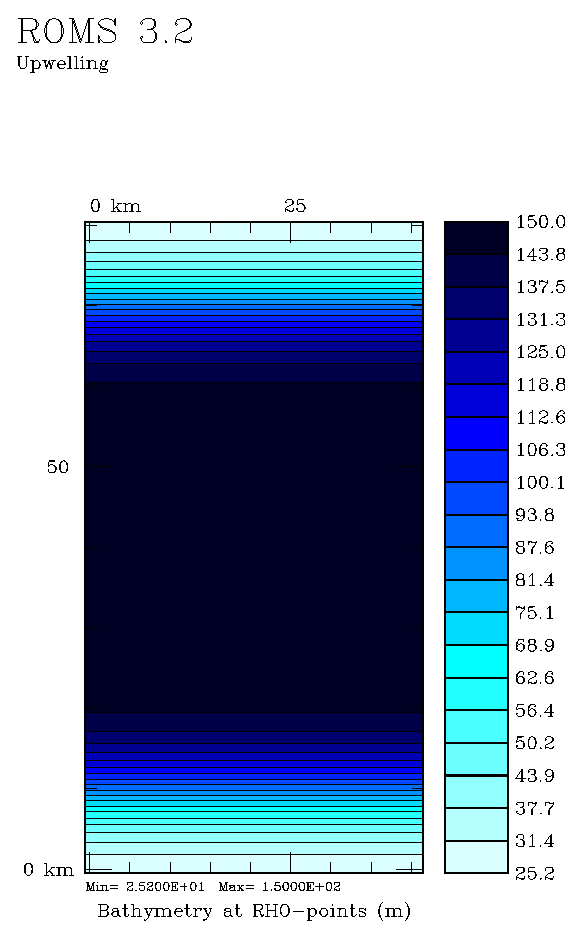
\includegraphics{pics/up1}
\end{picture}
\caption{The upwelling/downwelling bathymetry.}
\label{fsm1}
\end{figure}

\begin{figure}
\setlength{\unitlength}{10mm}
\begin{picture}(0,16)(-3.75,0)
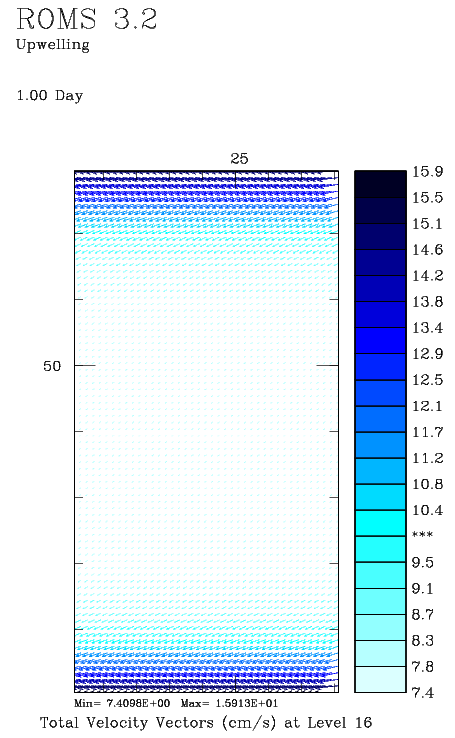
\includegraphics{pics/up2}
  \end{picture}
\caption{Surface velocities after one day, showing the flow to the
left of the wind (southern hemisphere).}
\end{figure}

\begin{figure}
\setlength{\unitlength}{10mm}
\begin{picture}(0,16)(0,0)
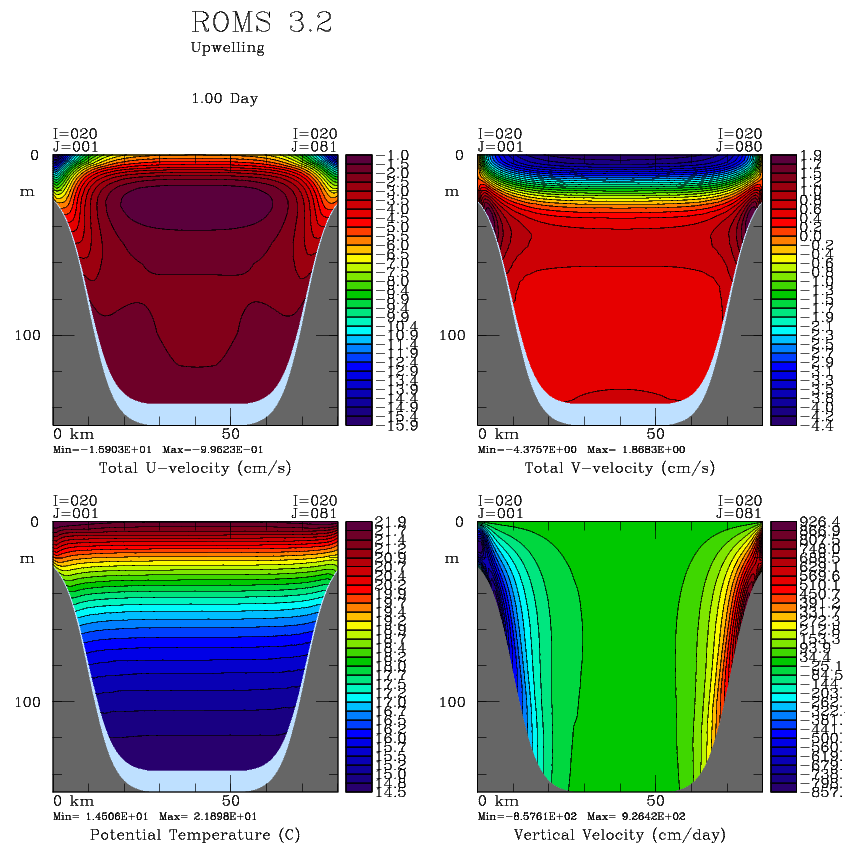
\includegraphics[width=6.5in]{pics/up3}
  \end{picture}
\caption{Constant $\xi$ slices of the $u, v, T$ and $w$ fields
at day 1.}
\end{figure}

\begin{figure}
\setlength{\unitlength}{10mm}
\begin{picture}(0,16)(0,0)
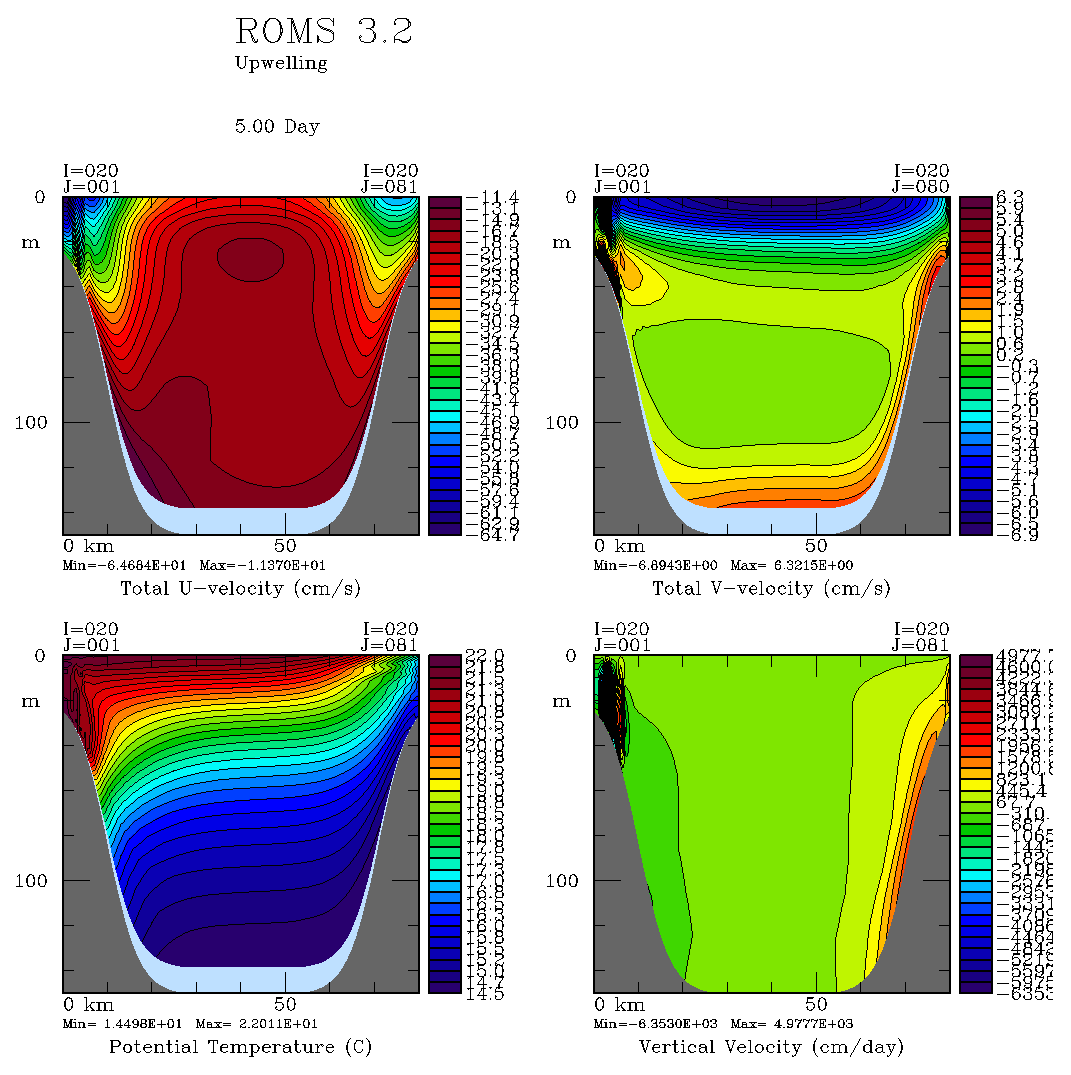
\includegraphics[width=6.5in]{pics/up4}
  \end{picture}
\caption{Constant $\xi$ slices of the $u, v, T$, and $w$ fields
at day 5.}
\label{fsm2}
\end{figure}

\subsection{Arctic example}
\label{ARCTIC}
The upwelling/downwelling examples is one in which all the start-up
fields are defined analytically.  The other extreme is one in which
everything is read from files, as in our Arctic simulations.
Figure \ref{fbath_arc} shows the bathymetry and the extent of this
domain. The grid is non-uniform, having more resolution close to
Alaska - a measure of grid spacing is shown in Figure
\ref{fgspace_arc}.

\begin{figure}
\setlength{\unitlength}{10mm}
\begin{picture}(0,16)(0,0)
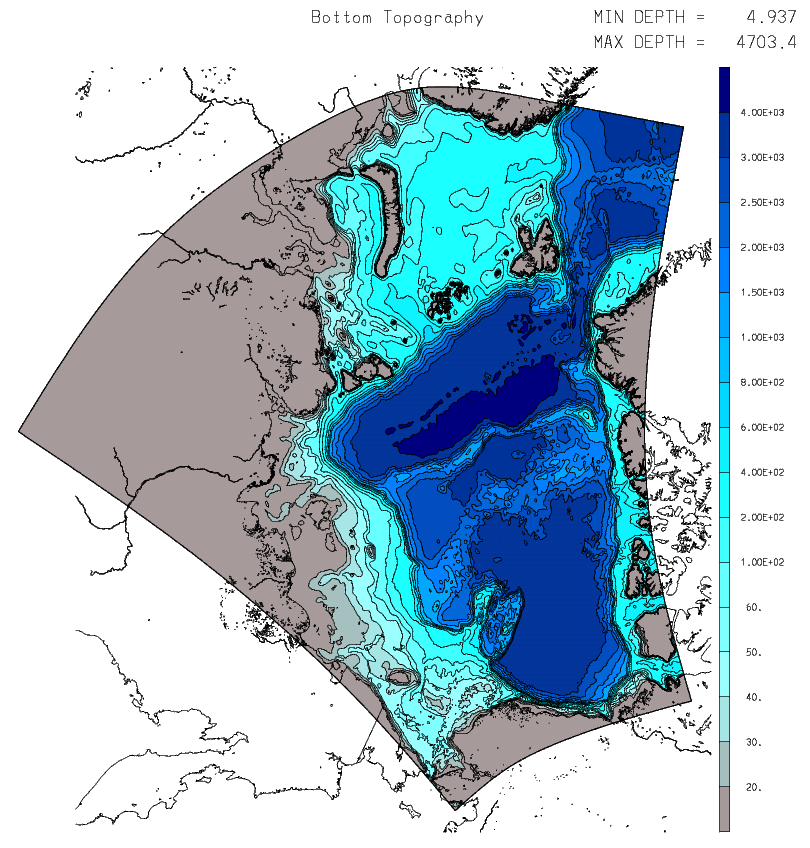
\includegraphics{pics/bath_Arc}
  \end{picture}
\caption{Bathymetry of the Arctic domain.}
\label{fbath_arc}
\end{figure}

\begin{figure}
\setlength{\unitlength}{10mm}
\begin{picture}(0,16)(0,0)
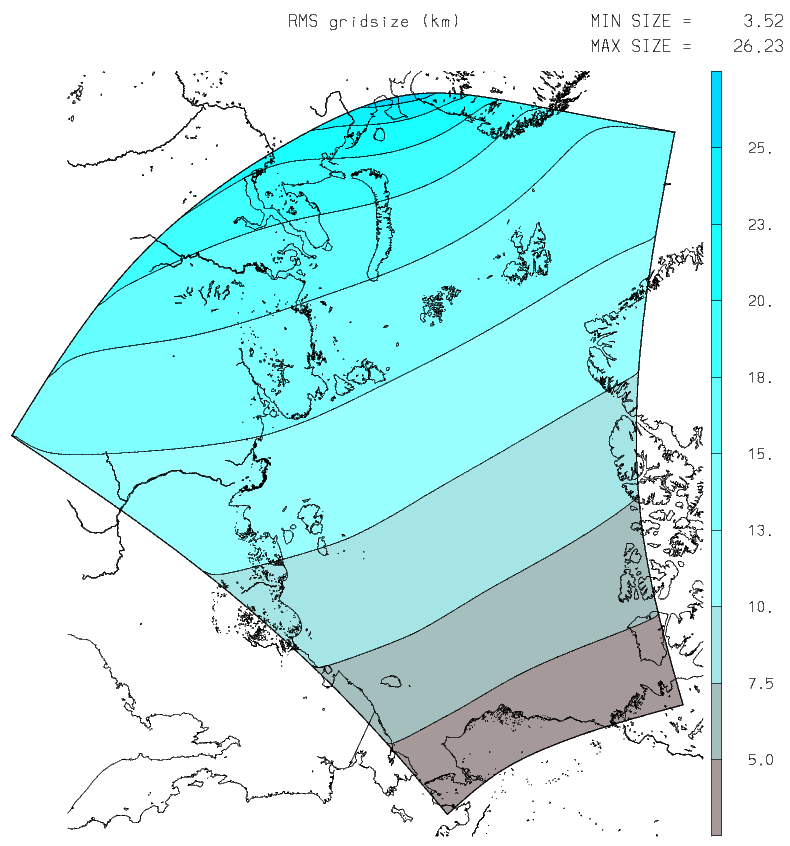
\includegraphics{pics/size_Arc}
  \end{picture}
\caption{Grid spacing of the Arctic domain.}
\label{fgspace_arc}
\end{figure}

\subsubsection{\code{arctic.h}}
The C preprocessor variable \code{ARCTIC} has been chosen to label
our Arctic domain---the header include file then becomes \code{arctic.h}:
\begin{verbatim}
/*
** svn $Id$
*******************************************************************************
** Copyright (c) 2002-2015 The ROMS/TOMS Group
**
**   Licensed under a MIT/X style license
**
**   See License_ROMS.txt
**
*******************************************************************************
**
**  Options for ARCTIC simulation
*/

#define NO_HIS
#define GLOBAL_PERIODIC
#define HDF5
#define DEFLATE
#undef PARALLEL_IN
#undef PARALLEL_OUT
#define PERFECT_RESTART

/* general */

#define CURVGRID
#define MASKING
#define NONLIN_EOS
#define SOLVE3D
#define SALINITY
#ifdef SOLVE3D
# define SPLINES_VDIFF
# define SPLINES_VVISC
# define RI_SPLINES
#endif
#define FLOATS
#define STATIONS
#undef WET_DRY

#define T_PASSIVE
#ifdef T_PASSIVE
# define ANA_BPFLUX        /* analytical bottom passive tracers fluxes */
# define ANA_SPFLUX 
# define ANA_PASSIVE
# define TRC_PSOURCE
# define ANA_TRC_PSOURCE
# define AGE_MEAN
# define PTOBC
#endif

/* ice */

#ifdef SOLVE3D
# undef CICE_MODEL
# ifdef CICE_MODEL
#  define SNOWFALL
#  define SNOW_FROM_RAIN
#  define INI_GLORYS_ICE
# endif

# define  ICE_MODEL
# ifdef ICE_MODEL
#  define ANA_ICE
#  define INI_GLORYS_ICE
#  define  OUTFLOW_MASK
#  define  FASTICE_CLIMATOLOGY
#  undef ICE_LANDFAST
#  define ICE_THERMO
#  define ICE_MK
#  define ICE_MOMENTUM
#  define ICE_MOM_BULK
#  define ICE_EVP
#  define ICE_STRENGTH_QUAD
#  define ICE_ADVECT
#  define ICE_SMOLAR
#  define ICE_UPWIND
#  define ICE_BULK_FLUXES
#  define ICE_CONVSNOW
#  define ICE_I_O
# endif
#endif

/* output stuff */

#define NO_WRITE_GRID
#undef OUT_DOUBLE
#ifndef PERFECT_RESTART
# define RST_SINGLE
#endif
#define AVERAGES
#define AVERAGES2
#ifdef SOLVE3D
# undef AVERAGES_DETIDE
# undef DIAGNOSTICS_TS
#endif
#undef DIAGNOSTICS_UV

/* advection, dissipation, pressure grad, etc. */

#ifdef SOLVE3D
# define DJ_GRADPS
#endif

#define UV_ADV
#define UV_COR

#ifdef SOLVE3D
# define TS_U3HADVECTION
# define TS_C4VADVECTION
# undef TS_MPDATA
#endif

#define UV_VIS2
#undef UV_SMAGORINSKY
#undef VISC_3DCOEF
#define MIX_S_UV
#define VISC_GRID

#ifdef SOLVE3D
# define TS_DIF2
# define MIX_GEO_TS
# define DIFF_GRID
#endif

/* vertical mixing */

#ifdef SOLVE3D
# define WTYPE_GRID

# undef LMD_MIXING
# ifdef LMD_MIXING
#  define LMD_RIMIX
#  define LMD_CONVEC
#  define LMD_SKPP
#  undef LMD_BKPP
#  define LMD_NONLOCAL
#  define LMD_SHAPIRO
#  undef LMD_DDMIX
# endif

# define GLS_MIXING
# undef MY25_MIXING

# if defined GLS_MIXING || defined MY25_MIXING
#  define KANTHA_CLAYSON
#  define N2S2_HORAVG
# endif
#endif

/* surface forcing */

#ifdef SOLVE3D
# define CORE_FORCING
# define BULK_FLUXES
# define CCSM_FLUXES
# define ARCTIC_MERRA_HACK
# if defined BULK_FLUXES || defined CCSM_FLUXES
#  define LONGWAVE_OUT
#  undef DIURNAL_SRFLUX
#  define SOLAR_SOURCE
#  define EMINUSP
#  undef ALBEDO_CLOUD
#  define ALBEDO_CURVE  /* for water */
#  undef ICE_ALB_EC92   /* for ice */
#  define ALBEDO_CSIM   /* for ice */
#  undef ALBEDO_FILE    /* for both */
#  undef LONGWAVE
# endif
#endif

/* surface and side corrections */

#ifdef SOLVE3D
# define SCORRECTION
# define NO_SCORRECTION_ICE
#endif

#ifdef SOLVE3D
# define ANA_NUDGCOEF
#endif

/* point sources (rivers, line sources) */

/* Using both for different regions */
#ifdef SOLVE3D
# define RUNOFF
# define TWO_D_TRACER_SOURCE
#endif

/* tides */

#define LTIDES
#ifdef LTIDES
# ifndef USE_DEBUG
#  define FILTERED
# endif
# define SSH_TIDES
# define UV_TIDES
# define ADD_FSOBC
# define ADD_M2OBC
# undef RAMP_TIDES
# define TIDES_ASTRO
# define POT_TIDES

# define UV_DRAG_GRID
# define ANA_DRAG
# define LIMIT_BSTRESS
# undef UV_LDRAG
# define UV_QDRAG
#else
# define UV_QDRAG
#endif

/* Boundary conditions...careful with grid orientation */

#define RADIATION_2D

/* roms quirks */

#ifdef SOLVE3D
# define ANA_BSFLUX
# define ANA_BTFLUX
#else
# define ANA_SMFLUX
#endif
\end{verbatim}
We've got masking, salinity, sea ice and the non-linear equation of state.
We want Laplacian viscosity on $\sigma$-surfaces, diffusion along constant
$z$-surfaces and the full non-linear, curvilinear momentum equations.

Notice that comments are allowed in this file as long as they are in
the C syntax. Also, conditionals are fine---some parts are only
wanted when \code{SOLVE3D} is on. Sources are now turned on in the
\code{ocean\_arctic2.in} file, while \code{RUNOFF} is still a
\code{cpp} option. We have both in this domain, using different
fresh water inputs for different parts of the domain.

\subsubsection{Arctic code chunks}
The \code{Apps/Arctic} directory contains the \code{ana\_}
family of include files for setting the bottom drag, the horizontal
nudging coefficients and the passive tracers.
Doing a search for \code{ARCTIC} shows up a few other bits of code. One
is in \code{output.F}, forcing a new station file after every
restart:
\begin{verbatim}
#ifdef ARCTIC
          CALL def_station (ng, .true.)
#else
          CALL def_station (ng, ldefout(ng))
#endif
\end{verbatim}
A better fix (someday) would be to allow the station files to be
numbered just like the averages files. Why not set \code{ldefout} to
be true? It is shared by many outputs, including the floats, and you
can only restart floats with \code{ldefout} set to false.

There is a hack in \code{grid\_coords.F} so that floats and stations
are placed at the correct $i,j$ position. Otherwise, the code to
find $i,j$ from longitude, latitude finds two boxes with the correct
range, one where I want it, the other at the same latitude, but
where the longitude jumps from 360 back to 0.

There is code in \code{set\_masks.F} to position the mask for
the ice outflow cells off the coast of Greenland.

Finally, there is a kludge in \code{step\_floats.F} for a
float reuse strategy, restarting them each year. Having a handy tag like
\code{ARCTIC} allows me to search for these little hacks later.

\subsubsection{Model domain}
A number of horizontal grid points was chosen to resolve the
domain at roughly 6 km near Alaska, less well across the basin. Values
for \code{Lm}, \code{Mm}, and \code{N} are:
\begin{verbatim}
          Lm == 688           ! Number of I-direction INTERIOR RHO-points
          Mm == 1088          ! Number of J-direction INTERIOR RHO-points
           N == 50            ! Number of vertical levels
\end{verbatim}
The vertical structure is set to our new favorite, using the new stretching:
\begin{verbatim}
  Vtransform == 2                          ! transformation equation
 Vstretching == 4                          ! stretching function

     THETA_S == 7.0d0                      ! surface stretching parameter
     THETA_B == 2.0d0                      ! bottom  stretching parameter
      TCLINE == 250.0d0                    ! critical depth (m)
\end{verbatim}

\subsubsection{Initial and boundary conditions}
The best ocean fields we knew of when setting this up are known as SODA, a
reanalysis from 1958 through 2008 by
\citet{Carton_2005}. There are global HYCOM fields for later years.
There are \code{Python} scripts to create
initial and boundary conditions from the SODA and HYCOM files. Snow and ice
initial conditions are set to uniform thicknesses where the SST is
cold, zero otherwise. Boundary conditions are assumed to be not
needed with the boundaries so far from the pack ice.

The side known as ``South'' is along the North Pacific.  The side
known as ``West'' is only open for a short bit in the North Pacific.
The last two boundaries are on the Atlantic and Canadian sides;
have our usual combination of radiation and nudging:
\begin{verbatim}
   LBC(isFsur) ==   Che     Che     Che     Che         ! free-surface
   LBC(isUbar) ==   Shc     Shc     Shc     Shc         ! 2D U-momentum
   LBC(isVbar) ==   Shc     Shc     Shc     Shc         ! 2D V-momentum
   LBC(isUvel) ==   RadNud  RadNud  RadNud  RadNud      ! 3D U-momentum
   LBC(isVvel) ==   RadNud  RadNud  RadNud  RadNud      ! 3D V-momentum
   LBC(isMtke) ==   Clo     Clo     Clo     Clo         ! mixing TKE

   LBC(isTvar) ==   RadNud  RadNud  RadNud  RadNud \    ! temperature
                    RadNud  RadNud  RadNud  RadNud \    ! salinity
                    Clo     Clo     Clo     Clo    \    ! inert(1)
                    Clo     Clo     Clo     Clo    \    ! inert(2)
                    Clo     Clo     Clo     Clo    \    ! inert(3)
                    Clo     Clo     Clo     Clo    \    ! inert(4)
                    Clo     Clo     Clo     Clo    \    ! inert(5)
                    Clo     Clo     Clo     Clo         ! inert(6)

! Ice boundary conditions

   LBC(isAice) ==   Clo     Clo     Clo     Clo         ! ice concentration
   LBC(isHice) ==   Clo     Clo     Clo     Clo         ! ice thickness
   LBC(isHsno) ==   Clo     Clo     Clo     Clo         ! snow thickness
   LBC(isTice) ==   Clo     Clo     Clo     Clo         ! ice temperature
   LBC(isApond)==   Clo     Clo     Clo     Clo         ! surface water
   LBC(isHpond)==   Clo     Clo     Clo     Clo         ! surface water
   LBC(isSig11)==   Clo     Clo     Clo     Clo         ! sigma-11
   LBC(isSig12)==   Clo     Clo     Clo     Clo         ! sigma-12
   LBC(isSig22)==   Clo     Clo     Clo     Clo         ! sigma-22
   LBC(isUice) ==   Gra     Gra     Gra     Gra         ! ice U-momentum
   LBC(isVice) ==   Gra     Gra     Gra     Gra         ! ice V-momentum

\end{verbatim}

\subsubsection{Forcing}
We are using the MERRA forcing files \citep{Rienecker_2011} and
computing the momentum, heat and salt fluxes from the atmospheric
conditions and the model's surface temperature. There are two
options, one provided by \code{bulk\_flux.F} and the other provided
by \code{ccsm\_flux.F}. We are using the second. We have \code{Python}
scripts for downloading MERRA so that the MERRA files can be used
as is, on their native grid, then interpolated by ROMS internally
to the domain at hand.  We have added a processing step to the MERRA
files so that only values from over the ocean are used - these are
extrapolated into the land points in the MERRA fields.

For fresh water input from land, we have the ARDAT fields for the
Arctic ocean \citep{Whitefield_2015}, which includes monthly river
temperature. These are applied as point sources to include the
effects of bringing in warm water. For the rest of the domain, we
are applying \citet{Dai_2009} as the \code{RUNOFF} field. Other
forcings include a nudging to sea surface salinity, a fastice
climatology from Andy Mahoney and tides from OTPS.

\subsubsection{ocean.in}
We use an internal time-step of 200 $s$ and an external time-step of 10
$s$. The horizontal viscosity and diffusion is:
\begin{verbatim}
        TNU2 == 5.0d0  5.0d0                    ! m2/s
       VISC2 == 25.0d0                          ! m2/s
\end{verbatim}

\subsubsection{Output}
The model writes voluminous information to standard out, as shown
for the \code{UPWELLING} case.  It also writes out NetCDF files for
restart, daily averages, three-hourly averages2, stations and floats.
Plots can be made from any of these files; some examples are shown
in Fig.\ \ref{fnep1}--\ref{fnep2} .

\begin{figure}
\setlength{\unitlength}{10 mm}
\begin{picture}(16,9)(0.0,0.4)
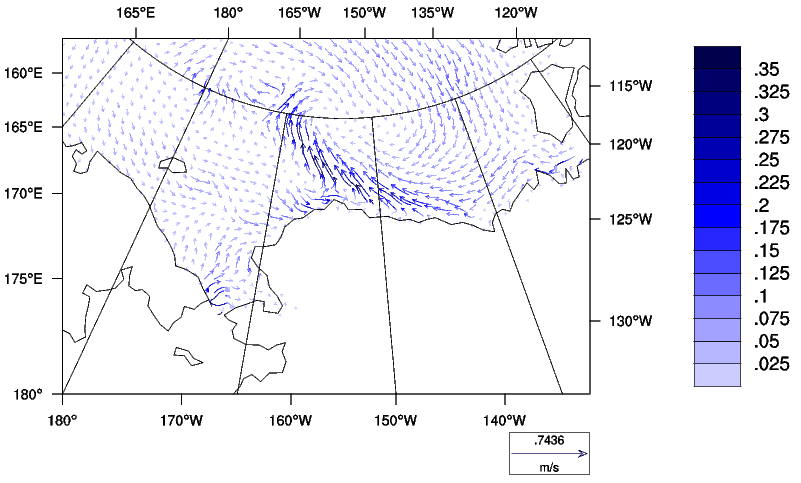
\includegraphics[width=16cm]{pics/usurf_Arc}
  \end{picture}
\caption{Surface velocity averaged over the month of June, 1986.}
\label{fnep1}
\end{figure}

\begin{figure}
\setlength{\unitlength}{10 mm}
\begin{picture}(16,12)(0.0,0)
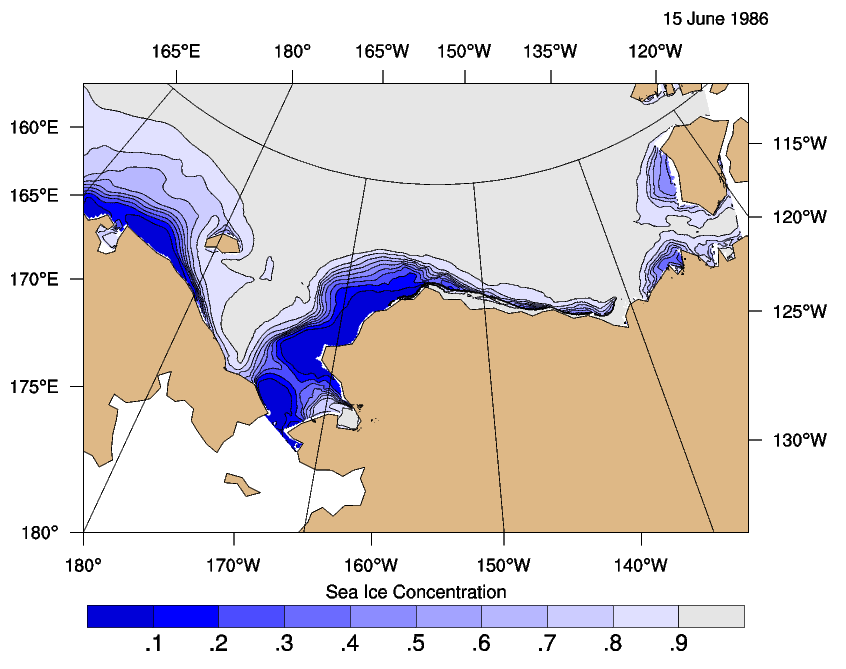
\includegraphics[width=16cm]{pics/aice_Arc}
  \end{picture}
\caption{Ice concentration averaged over the month of June, 1986.}
\end{figure}

\begin{figure}
\setlength{\unitlength}{10 mm}
\begin{picture}(16,18)(0.0,0)
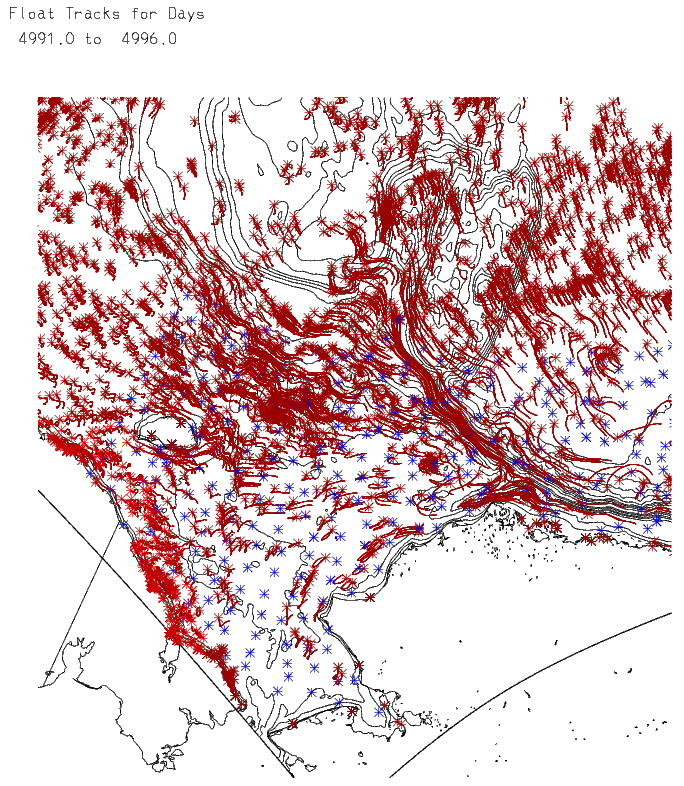
\includegraphics[width=16cm]{pics/float_Arc}
  \end{picture}
\caption{Five-day tracks of some surface floats, showing the starting
positions in blue.}
\label{fnep2}
\end{figure}

